\documentclass[11pt]{report}
\usepackage{baththesis}
\usepackage{graphicx}
\usepackage{caption}
\usepackage{amsmath}
\usepackage{subcaption}
\usepackage{verbatim}
\usepackage[inline]{enumitem}
%\usepackage{amsfonts}
\usepackage{url}
\usepackage{natbib}
\usepackage[hmargin=3cm,vmargin=2cm]{geometry}
%\usepackage{mathpazo}
%\usepackage{eulervm}
\usepackage[usenames,dvipsnames,svgnames,table]{xcolor}
\usepackage[]{todonotes}
\usepackage{tikz}
\usetikzlibrary{arrows}
\usepackage[]{todonotes}

\def\mnote#1{\todo[color=Goldenrod,size=\scriptsize]{Matt: #1}}
\def\jnote#1{\todo[color=CornflowerBlue,size=\scriptsize]{Julian: #1}}
\def\snote#1{\todo[color=WildStrawberry,size=\scriptsize]{Steve: #1}}
\definecolor{light-gray}{gray}{0.95}

\usepackage{listings}
\lstset{ %
   language=prolog,
%  frame=l,                     % adds a frame around the code
   basicstyle=\footnotesize\ttfamily,  % use courier
   breaklines=true,
   xleftmargin=0.5em,
   aboveskip=0.5em,
   belowskip=0.5em,
%  belowcaptionskip=5em,
   numbers=left,
   backgroundcolor=\color{light-gray},
   frame=single,
   framerule=0pt
}

\setlength{\jot}{0pt}
\def\mylabel#1{\tikz[remember picture]\node(#1){};}
\def\myref#1#2#3{\begin{tikzpicture}[remember picture]
\node[draw,rounded corners] (#2){\begin{minipage}{\textwidth}\raggedright#3\end{minipage}};
\draw[overlay,-triangle 45,thick,gray](#2.west)--(#1.west);
\end{tikzpicture}}

\title{Building Abstractable Story Components with Institutions and Tropes}
\author{Matt Thompson}
\degree{EngD Digital Media}
\department{Department of Computer Science}
\degreemonthyear{October 2016}
\norestrictions


\begin{document}
\maketitle
\renewcommand{\abstractname}{Related Presentations and Publications}
\begin{abstract}
  The following list includes all conference presentations and papers published by the author which are related to this report.
  \begin{itemize}
  \item\textbf{[HSWI@ESWC 2014] Artfinder: A Faceted Browser for Cross-Cultural Art Discovery} Matt Thompson, Julian Padget and Steve Battle, Human Semantic Web Interaction Workshop, European Semantic Web Conference, May 2014, Crete, Greece.
  \item\textbf{[DHIS 2015] Every Object Tells a Story} Matt Thompson, Julian Padget and Steve Battle, Digital Heritage Meets Interactive Storytelling 2015 (conference presentation), April 2015, York UK.
  \item\textbf{[AISB 2015] An Interactive, Generative Punch and Judy Show Using Institutions, ASP and Emotional Agents} Matt Thompson, Julian Padget and Steve Battle, AISB AI \& Games Symposium, April 2015, Canterbury, UK.
  \item\textbf{[CMN 2015] Governing Narrative Events with Institutional Norms} Matt Thompson, Julian Padget and Steve Battle, Sixth International Workshop on Computational Models of Narrative, May 2015, Atlanta, USA.
  \item\textbf{[COIN@IJCAI 2015 (submitted)] An Interactive, Generative Punch and Judy Show Using Institutions, ASP and Emotional Agents} Matt Thompson, Julian Padget and Steve Battle, International Workshop on Coordination, Organisation, Institutions and Norms in Multi-Agent Systems, July 2015, Buenos Aires, Argentina.
  \end{itemize}
\end{abstract}
\clearpage
\tableofcontents
\clearpage

\chapter{Introduction}
\label{cha:introduction}

\chapter{Literature Review}
\label{cha:literature-review}
This research covers a large number of fields of study, therefore an extensive literature review covering these fields is needed. This section starts with a look at the field of \emph{narratology}, or narrative theory, to gain some insights into the themes and components that make up stories. We examine different formalisms that have been created for narrative and which themes and motifs recur in order to better generate stories for ourselves.

Additionally, computers have the potential to introduce a new type of storytelling. Though computer games offer increasingly immersive interactive worlds, the form of narrative they use remains much the same: linear. A player may be able to interact with elements of a game, but the story itself remains unchanged.

Chris Crawford refers to a new possible form of narrative as ``Interactive Storytelling'' \citep{crawford2012chris}. Though researchers and game designers have made great strides towards realising this new artform, little has been produced to capture the public imagination.

In order to better inform any implementation of interactive narrative, I begin with an examination of the field of classic narrative theory. Following from this is a look at the emerging research in interactive and generative narrative and their implementations.

As part of the examination of implementations of interactive narrative, I especially focus on agent-based systems. The section concludes with an overview of emotional models that can be used to model distinct characters using agents.

\section{Narratology}\label{sec:narratology}
Narratology is a deep field with many sub-fields. This review examines the parts of it that might best inform the modelling of narrative by computers, as well as the construction of interactive narrative.

Structuralist formalisms of narrative attempt to explain how stories work by dividing them into commonly occuring themes and motifs. This is a natural fit to the modelling of narratives by computer, especially if using an ontology. Our overview of narratology starts with structuralism for this reason.

The second part of our overview of narratology examines more recent work done on ``cybertext'' and experimental narrative in the interactive age. From this examination of recent research into non-linear narratives we can learn how to better construct interactive narratives for games or simulations.

\subsection{Structuralist formalisms of narrative}
Attempts to organise recurring themes, roles and motifs of narrative go back at least a century. The Aarne-Thompson tale-type index \citep{aarne1987types}, first published in 1910 and later refined by Stith Thompson in 1928 and 1961, is well known amongst folklorists as a classification and analysis method for traditional folktales and myths. Aarne-Thompson's index is a taxonomy of tale themes, arranging tales into categories such as \emph{animal tales} and \emph{jokes and anecdotes}, and then sub-categories (\emph{tales of magic} and \emph{numskull [sic] stories} being two examples). This taxonomy is only two levels deep however, and only serves as a useful way to categorise individual stories or tales. In order to break down and analyse components of tales, we must dig deeper.

In \emph{Structural Anthropology}, Claude L\'{e}vi-Strauss seeks to discover why myths and legends are so similar across cultures and history \citep{levi2008structural}. He concludes that there are global laws that govern the way in which people create stories, therefore these laws can be modelled as a set of rules for describing myths.

His theory is that myths describe opposing forces which are resolved through mediation. The example he gives in \emph{Structural Anthropology} describes how Native American legends often contain `trickster' characters in the form of ravens or coyotes. As scavenging animals, these tricksters symbolically act as mediators between life and death.

Like much of early narrative theory, there is no rigorous evaluation of L\'{e}vi-Strauss' ideas, leaving them feeling a little too opinionated and arbitrary. While interesting, L\'{e}vi-Strauss' ideas bring us no closer to developing a formal model of narrative structure. For that, we must go even further back in time, and turn to Vladimir Propp.

\subsubsection{Propp's Morphology of the Folktale}\label{sec:propp}
Propp's seminal work ``The Morphology of the Folktale'' \citep{propp1968morphology}, though first published in 1928, is still a widely-used formalism for researchers and game designers looking to generate narratives procedurally. Propp identifies recurring characters and motifs in Russian folklore, distilling them down to a concise set of rules with which to describe stories.

In this formalism, characters have \emph{roles}, such as \emph{hero}, \emph{villain}, \emph{dispatcher}, \emph{false hero}, and more. Characters performing a certain role are able to perform a subset of \emph{story functions}, which are actions that make the narrative progress. For example, the \emph{dispatcher} might send the \emph{hero} on a quest, or the \emph{victim} may issue an \emph{interdiction} to the \emph{villain}, which is then \emph{violated}.

Propp defines a total of 31 distinct story functions, each of which is given a number and symbol in order to create a succinct way of describing entire stories. Examples of such functions are:

\begin{itemize}
  \item One of the members of a family absents himself from home: \emph{absentation}.
  \item An interdiction is addressed to the hero: \emph{interdiction}.
  \item The victim submits to deception and thereby unwittingly helps his enemy: \emph{complicity}.
  \item The villain causes harm or injury to a member of the family: \emph{villainy}.
\end{itemize}

Each of these functions can vary to some degree. For example, the \emph{villainy} function can be realised as one of 19 distinct forms of villainous deed, including \emph{the villain abducts a person}, \emph{the villain seizes the daylight}, and \emph{the villain makes a threat of cannibalism}.

These functions are enacted by characters following certain roles. Each role (or \emph{dramatis personae} in Propp's definition) has a \emph{sphere of action} consisting of the functions that they are able to perform at any point in the story. Propp defines seven roles that have distict spheres of action: \emph{villain}, \emph{donor}, \emph{helper}, \emph{princess}, \emph{dispatcher}, \emph{hero}, and \emph{false hero}.

Though Propp defines each \emph{dramatis personae} as being distinct (characters can only play one role at a time), it is simple to extend the idea to allow for overlapping roles. For example, a victim could also be a donor, so the set of functions they can perform would be the union of both the victim and donors' permitted function sets. Propp does not explore this possibility in \emph{The Morphology of the Folktale}, however.

\begin{figure}[!t]
\centerline{
\includegraphics[height=0.4in]{propp1.png}}
\caption{One Propp function following another} \label{fig:propp1}
\end{figure}

\begin{figure}[!t]
\centerline{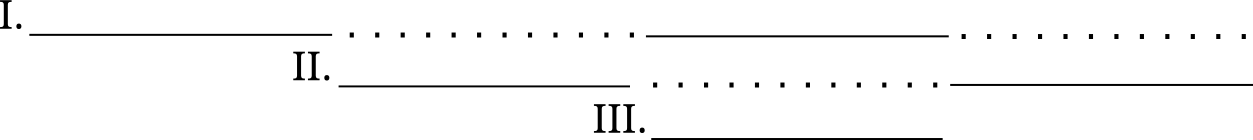
\includegraphics[height=0.6in]{propp2.png}}
\caption{Multiple simultaneous functions} \label{fig:propp2}
\end{figure}


In a typical story, one story function will follow another as the tale progresses in a sequential series of cause and effect (figure \ref{fig:propp1}). However, Propp's formalism also allows for simultaneous story functions to be occuring at once (figure \ref{fig:propp2}).

% More is needed, I reckon

% time is short: only put this in if really needed
%\subsection{Fabula and Syuzhet}
%\subsection{Narreme}

%\subsection{Polti's thirty-six dramatic situations}

%\subsection{Booker's seven basic plots}
% Reference prior work from Wikipedia article

% Egri's premises, Polti's dramatic situations (see ICIDS 2011, page 123)
% Look into Roland Barthes' stuff (narremes in 1966)

% Maybe shunt this to the research plan section?
%\subsection{Tropes in narrative}

% Tropes

\subsection{Cybertext: Experimental narrative and digital media}\label{sec:media}
The rise of the Web in the 1990s brought with it great interest in the future of narrative in cyberspace. Aarseth's groundbreaking work, \emph{Cybertext} \citep{aarseth1997cybertext} describes the creation of a new form of narrative, for which he coins the term \emph{ergodic literature} (from the Greek words \emph{ergon} and \emph{hodos}, meaning `work' and `path'). In this new form of narrative, some amount of work or effort is required by the reader in order to traverse the path that the story takes.

% scriptons/discourse textons/fabula (Bal 1997)
Aarseth makes a distinction between the narrative as written by the author, and the way in which it is traversed by the reader, calling the former \emph{textons} and the latter \emph{scriptons}. In ergodic literature, the \emph{scripton} is produced by the effort that the reader goes through in interpreting the \emph{texton}. In the context of a game, it is as though the game interface is a gateway that allows access to the narrative at different times. Using classical music as a metaphor, the texton can be thought of as the \emph{score}, and the scripton the \emph{performance}.

% Make sure you actually made this assertion
In section \ref{sec:generative-and-interactive-narrative}, we assert that how generative a narrative is and its level of interactivity are two different variables in an experimental narrative. However, Aarseth identifies seven different methods of story traversal: \emph{dynamics, determinability, transiency, perspective, access, linking and user function}.

\begin{itemize}
\item\textbf{Dynamics} describe whether or not the content and number of scriptons changes. In a simple, static story with branching choices (such as in a \emph{Choose your own adventure} story), both the number of textons and scriptons are fixed, since all paths have been written out beforehand. A dynamic story would still have a fixed number of textons, but the scriptons would be generated as the user traverses the path of the narrative.
\item\textbf{Determinability} is how deterministic the narrative is, whether or not the same interactions will result in the same scripton being produced.
\item\textbf{Transiency} means to what extent scriptons are produced as time flows, or whether user interactions are required to produce them.
\item\textbf{Perspective} is whether or not the user/reader plays a role as a character in the narrative.
\item\textbf{Access:} if a user has access to all scriptons at any point in traversing the narrative, or whether their access is restricted.
\item\textbf{Linking} means whether or not parts of the scripton are linked to other parts, and whether these links are conditional (if they rely on a user having already traversed part of the scripton).
\item\textbf{User functions:} the functions the user uses to traverse the text. This could be interpretive (which is implicit in any traversal of the text), explorative (traversing the scripton according to whim) or configurative (specifying parts of the scripton in advance), for example.
\end{itemize}


% Ugh, this is all so arbitrary. Go on to describe Aarseth's PCA of these variables and explain why you don't think it's a good fit.

By performing correspondence analysis (a process similar to principle component analysis) on a diverse corpus of 23 texts ``\emph{ranging from ancient China to the Internet}'', Aarseth filters these seven variables down into two numerical axes which account for 49 percent of the variation between stories. Using these axes, he groups classic tales such as \emph{Moby Dick} and more experimental narratives such as William Gibson's \emph{Agrippa} and Michael Joyce's \emph{Afternoon}. By grouping these stories into categories, he intends to show how emerging media are enabling new types of story.

Chris Crawford's \emph{Chris Crawford on Interactive Storytelling} \citep{crawford2012chris} provides a scathing assessment of the relationship between narrative theory and computer science. A veteran of the games industry, he argues that `soft' science theories such as those of Aarseth et al are entirely removed from `hard' science, and are therefore an example of bubble intellectualism and impossible to implement. 

Crawford himself provides a useful examination of experimental narrative in computer games, defining interactivity as:

\begin{quote}
A cyclic process between two or more active agents in which each agent alternately listens, thinks, and speaks.
\end{quote}

He argues that for game narratives to be truly interactive, they must be more social. Characters in a story must be able to react with the player as though they were people in real life. In turn, the player should have some degree of freedom in the way in which they interact. Rather than presenting branching story points as choices, a better way to interact would be socially, through talking to agents in the game. This is the approach that Fa\c{c}ade takes \citep{mateas2003faccade}, which Crawford acknowledges as the most successful attempt at interactive storytelling to date. A detailed description of Fa\c{c}ade's implementation appears in section \ref{sec:modelling-agents}.

In order to determine whether Crawford's assertion that narratology research is too far removed from its practical implementations to be of use, we next provide an overview of these implementations and their underlying research. Has narrative theory research informed the creation of computer-generated or interactive narrative at all, or do they all take approaches grounded in computer science and artificial intelligence? If narrative theory has not been used, then we must ask another question: why not?

% Murray
% Laure-Ryan

\section{Implementations of experimental narrative}\label{sec:generative-narrative}
% Cite (Crawford interview guy) as saying a modular approach is desirous, with:
% Brian Magerko’s actors
% Mateas' drama manager
% ASAPS could supply a meta-narrative structure
% Aylett/Louchart’s agents would take over, combined with Michael Young’s work, Mark Riedl’s sequencing and Jichen Zhu’s story generation. Ideally, artists could supply elements in this way, too, for example some of Toni Dove’s work.
% LOOK INTO THE ABOVE
% There's also a lot more to look at in that interview.

% What is generative narrative?
Although Aarseth describes seven variables influencing story type in \emph{Cybertext}, he distills these down into two axes that can be used to group together types of narrative. Though Aarseth's correspondence analysis is used to arrange texts in the corpus along \emph{numerical\/} axes, research into experimental narrative implementations can generally be classed as \emph{generative} narrative, \emph{interactive} narrative, or both. For this reason, the two axes identified by Aarseth are likely to correspond to these two variables. 

Generative narrative is the procedural generation of stories by a computer program. The author describes the story domain using characters, scenarios or both, and the narrative is `generated' by filling in the details. Often, it is more than just the details that are filled in, as the entire story can be produced from the smallest of specifications.

An interactive narrative is a story which changes according to the interactions of the player or reader. The player may be forced to make decisions as they play through the narrative which lead to different story paths. Alternatively, a narrative may be both interactive and generative if stories are created from the actions of the player.

While much of the literature is devoted to either purely generative narrative (such as the generative grammar-based approaches) or purely interactive narrative (such as pre-authored planning-based systems), there are many approaches that lie somewhere between the two. In this section I examine the approaches taken in the literature, and to what extent they are generative, interactive or both.

% Are later stuff hybrid approaches? ABL, Riedl & Young's narrative planning?

\subsection{Generative grammar approaches}
Inspired by Chomsky's theories of generative grammar \citep{chomsky1968sound}, researchers in generative narrative strive to build their own `universal grammar' for narrative.

\begin{figure}[!t]
  \begin{center}
  \begin{enumerate}
    \item $\texttt{Attempt}\rightarrow \texttt{Plan} + \texttt{Application}$\\
           $\qquad\Rightarrow\texttt{MOTIVATE(Plan, Application)}$
    \item $\texttt{Application}\rightarrow\texttt{(Preaction)*} + \texttt{Action} + \texttt{Consequence}$\\
           $\qquad\Rightarrow\texttt{Allow(AND(Preaction,Preaction,...),}$\\
           $\qquad\{\texttt{CAUSE | INITIATE | ALLOW}\}\texttt{(Action,Consequence)}$
  \end{enumerate}
  \end{center}

  \caption{Example rules from Rumelhart's story grammar}\label{fig:rumelhart}
\end{figure}

\citet{rumelhart1975notes} is one early and influential model for the grammatical generation of natural language. Figure \ref{fig:rumelhart} shows two example rewrite rules from this grammar. The `+' symbol denotes items happening in a sequence, the `\textbar' showing possible alternatives. `*' denotes one or more item being generated. Capitalised words (such as ALLOW, MOTIVATE, etc) describe relationships between items. For example, MOTIVATE is a relationship between a character's thought and their reaction to that thought.

This generative grammar approach can be seen in systems such as Pemberton's GESTER \citep{pemberton1989modular}, which generates stories based on a grammar synthesised from old French epic tales. \citet{lang1999declarative} describe a declarative model for narrative, consisting of lists of first-order predicate calculus expressions. These expressions describe events, states, goals and beliefs which combine to form a narrative. More specifically, it combines:

\begin{itemize}
  \item A \textbf{grammar interpreter} to search for a sequence of grammer rewrites which would produce a convincing narrative.
  \item A set of \textbf{temporal predicates} to describe the occurence of events over time and enforce temporal constraints on story components.
  \item A \textbf{world model} which describes the set of actions that characters may perform and fluents that may alter over the course of the narrative.
  \item A \textbf{natural language output unit}, which takes the sequence of events produced by the story grammar and converts it into readable natural language sentences.
\end{itemize}

This combination of using a grammar interpreter, world model and natural language output unit is especially common amongst generative grammar approaches.

While generative grammar approaches may be effective for procedurally creating prose, they are less well suited to the creation of \emph{interactive} narratives. Once the grammar rewrite rules are specified, the user is entirely passive, unable to affect the way in which the story is bein generated. For this to happen, the narrative needs to be part of a system that reacts to the actions of the user, such as a computer game.

\subsection{Author modelling and planning approaches}

% narrative intelligence [12] from riedl's paper
% i-storytelling system [6]
% universe [9]
% wehrauch 1997, Bates 92: drama manager
% facade?
One problem with the generative grammar approaches is that there is little balance between author and character story generation. Everything that can happen in the story is written down in the rewrite rules. It leaves little room for character models, or having characters with unique personalities and plans. In order to make a rich generative narrative, a balance must be reached between an authored story strucure and character-generated dialogue and plans.

One common method for balanced story generation is through planning: searching through sequences of possible actions in order to find one that help achieve a goal. Planners can be used both as a way for the narrative to reach an end goal, and for the characters inside of a narrative to attempt to achieve their own desires.

\citet{young1999notes} argue that planners are a good method for regulating plot, later creating an architecture to integrate a planner with character agents in an interactive game environment \citep{young2004architecture}.

\begin{figure}[!t]
\begin{quote}
  ONCE UPON A TIME GEORGE ANT LIVED NEAR A PATCH OF GROUND. THERE WAS A NEST IN AN ASH TREE. WILMA BIRD LIVED IN THE NEST. THERE WAS SOME WATER IN A RIVER. WILMA KNEW THAT THE WATER WAS IN THE RIVER. GEORGE KNEW THAT THE WATER WAS IN THE RIVER. ONE DAY WILMA WAS VERY THIRSTY. WILMA WANTED TO GET NEAR SOME WATER. WILMA FLEW FROM HER NEST ACROSS THE MEADOW THROUGH A VALLEY TO THE RIVER. WILMA DRANK THE WATER. WILMA WASN'T THIRSTY ANYMORE.

GEORGE WAS VERY THIRSTY. GEORGE WANTED TO GET NEAR SOME WATER. GEORGE WALKED FROM HIS PATCH OF GROUND ACROSS THE MEADOW THROUGH THE VALLEY TO A RIVER. GEORGE FELL INTO THE WATER. GEORGE WANTED TO GET NEAR THE VALLEY. GEORGE COULDN'T GET NEAR THE VALLEY. GEORGE WANTED TO GET NEAR THE MEADOW. GEORGE COULDN'T GET NEAR THE MEADOW. WILMA WANTED TO GET NEAR GEORGE. WILMA GRABBED GEORGE WITH HER CLAW. WILMA TOOK GEORGE FROM THE RIVER THROUGH THE VALLEY TO THE MEADOW. GEORGE WAS DEVOTED TO WILMA. GEORGE OWED EVERYTHING TO WILMA. WILMA LET GO OF GEORGE. GEORGE FELL TO THE MEADOW. THE END.
\end{quote}
\caption{Example TALE-SPIN output}\label{fig:tspin}
\end{figure}

Lebowitz' UNIVERSE system \citep{lebowitz1985story} focuses on the creation of believable characters, using `plot fragments', or short plans, to generate story outlines for soap operas.

In Cavazza et al's I-Storytelling system \citep{cavazza2001characters}, plans are formulated by creating Hierarchical Task Networks (HTNs) consisting of goals, subgoals, and the actions required to achieve those goals.


James Meehan's TALE-SPIN \citep{meehan1977tale} is an influential early approach to story generation using planning. In TALE-SPIN, the author describes a story domain, its characters and their goals, and a natural language story is produced as output. It works by using a problem-solver to resolve each character's goals over the story domain. Figure \ref{fig:tspin} is an example of TALE-SPIN's output.

TALE-SPIN's strong planning component is evident in the reading of its output. Sentences are terse, with one event leading directly to another in order to achieve some goal. One problem with this character-led approach is that the goals of the author are not necessarily taken into account. If the author intends for a character to die at some point in the story, it seems unnatural for a character to have the goal of dying to fulfill this intention.

 Turner criticises TALE-SPIN's stories as seeming ``pointless and somewhat boring'' \citep{turner1986thematic}, going on to create the MINSTREL system for story generation \citep{turner1993minstrel}. Using the legendary world of King Arthur's court as a story domain, MINSTREL strives to generate stories with an authorial purpose.

MINSTREL attempts to address TALE-SPIN's shortcomings by introducing two types of schema: author-schemas and character-schemas, both of which combine to represent the elements of a story. The author-schemas describe the goals of the author of the system, allowing story creators more control over the structure and content of their narrative. This allows authors to specify a `point' or moral to their story, something that is not possible to achieve with TALE-SPIN. Character-schemas describe character-level goals in a similar manner to those of TALE-SPIN's.

The comparison of TALE-SPIN and MINSTREL highlights a challenge that has dominated story generation for decades: the balance of \emph{character} and \emph{plot}. Especially with approaches based on multi-agent systems, the regulation of character actions to conform to an underlying theme or structure is a challenging problem.

However, modelling characters with agents is a promising approach to take in order to gain a story which is both generative and interactive. In such a system, an author can specify the story world and character models, creating the `big picture', and the agents would be able to fill in the details (such as dialogue, sub-plots, and relationships).

An apt metaphor would be that of animation. In large animation studios such as Disney, the lead animator draws the key frames of a sequence, and a team of other animators works to fill in the gaps in between. This is what the combination of a managed narrative with agents could achieve: the author would be the `lead animator' in such a system, with the agents being the assistants.

So far into this literature review, we have some idea of where a promising approach may lie. However, the implementations until now have still focused mainly on \emph{generation\/}, and little on \emph{interaction\/}. Character models have been mentioned, but these do not react in real time to a user. For that, we need a multi-agent system.

% Expand!



% 3 papers from Lang: Rumelhart, Lebowitz, Talespin
% Lang uses Propp (actually: no). Who else?
% Prada et al use Propp: Teatrix: Virtual Environments for Story Creation 2000
% Szilas uses more recent narrative theories: Interactive Drama on Computer: Beyond Linear Narrative 1999
% Story grammar approaches
% Using Propp/Strauss/Thompson
% Talespin
% Minstrel
% Geist
% Riedl
% Storymaking project
% IRIS project
% MAS approaches
% recent approaches
% BRUTUS? MEXICA?

% ELIZA?
% Galatea
% Facade evolved from the OZ project
% Thespian (+ other agent/BDI approaches)
% Twinery?

\subsection{Modelling characters with agents}\label{sec:modelling-agents}
Once a story is created by simulating the characters of a story as intelligent agents, it can become truly interactive: the agents can react to the player in order to create a narrative.

Using an agent-based approach to modelling characters in a story has many advantages. Perhaps the largest is that it simplifies the creation of story details for an author. The writer of an experimental generative narrative need only describe the outline of a story and the characters in it, then the agents can take care of the small decisions of the narrative that have no bearing on its structure.

For example, conversational agents could be used to work out the dialogue of a story amongst themselves, so long as the dialogue conforms to the narrative events described by the author.

Riedl and Young make much use of agents and planners in their work, for both interactive and generative narrative. Addressing the problem of balancing character believability with plot coherence, they present a planner-based solution for story generation \citep{riedl2004intent}. Their planner is described as an `intent-driven partial order causal link' planner, planning actions for agents in a multi-agent system based on causality and intention.

In this case, \emph{intention} refers to a component of agents based on the Belief Desire Intention (BDI) framework. Their planner observes the actions of the agents in the system and infers their intentions.

\paragraph{Thespian} \citep{si2005thespian} is an interactive drama system for learning language and cultural awareness. It is built on PsychSim, a multi-agent system for social simulation based on Partially Observable Markov Decision Problems (POMDPs) \citep{marsella2004psychsim}.

Thespian agents are comprised of a set of goal state features, a set of event state features, policies, available actions and recursive beliefs about themselves and other characters appearing in the same story. The Thespian system itself only has one type of goal: to maximise or minimise a goal state variable.

The agents act out their parts in turn. Turn-taking is based on agent arousal, with the most aroused agent getting the next turn if it wants to speak. When an agent selects an action for its next turn, it uses a lookahead process to consider how other agents will respond to each action.

The story is authored by having the creator put in each characters' goal weights as parameters. Each agent has a \emph{personality profile} that consists of its \emph{goals}, and certain \emph{weights} for those goals. It uses a \emph{fitting algorithm} to go through all of the characters and determine their behaviour based on the agent's goals. It does this by calculating constraints to agent behaviours based on their goal weights. This helps to automate the authoring of characters.

The overall arc of the story is controlled using \emph{dynamics functions}, which define how characters' actions can affect the world.

Thespian is designed with ease of character and story authoring in mind. Character authoring is automated in the fitting process of character roles to story. Building a story environment still requires some programmer effort, however, and is split into three steps:

\begin{enumerate}
  \item Create a list of possible actions each character can perform, and a list of relevant goals.
  \item Check each pair of goal and action to see if a function for achieving this in the story has already been defined.
  \item If not, the function for achieving the goal must be written.
\end{enumerate}

Character authoring similarly follows three steps:

\begin{enumerate}
  \item The author sets the initial conditions for each character. They can do this by selecting one of a set of predefined agents.
  \item The author defines a desired path for the story by specifying a sequence of actions that should happen at some point in the story.
  \item The fitting process uses these paths to guide the creation of the characters from their goal weights.
\end{enumerate}

Though POMDPs are useful in that they give the agents a `theory of mind' they are not grounded in psychological theory of human reasoning, as with Belief-Desire-Intention (BDI). This means that extending them with human traits such as emotions could be difficult.

For example, an agent's ability to plan is very limited with POMDPs. They are either purely reactive or try to optimise some variable based on limited lookahead. With BDI agents, different plans can be followed according to an agent's (for example) emotional state at the time.

\paragraph{The OZ project}
Carnegie Mellon University's OZ project \citep{mateas1999oz} is one of the first major research efforts towards creating interactive drama using agents as characters. A dramatic structure is given to the narrative by means of a \emph{drama manager}, which is able to see all of the actions occurring in the storyworld and can change anything in order to create a better experience for the user.

Ideas from the OZ project were later developed into what would become Fa\c{c}ade.

% Say that this work was the precursor to Facade

\paragraph{Fa\c{c}ade}
Mateas and Stern's \emph{Fa\c{c}ade} has players interact with the characters of the story through natural language. In this game, the player attends the party of a young couple (Grace and Trip) celebrating their wedding anniversary. As the course of events unfold however, the player learns that all is not as happy as it seems.

The player interacts with the characters by typing in natural language sentences, to which Grace and Trip respond. Though the characters are implemented through agents, the story is controlled using a drama manager. In all, their system consists of using NLP, a novel character authoring language and a novel drama manager to create an interactive narrative.

Several custom-designed languages were used to create the game, including a language called `A Behaviour Language' (ABL) for the agents and a special language for the sequencing of the beats. ABL represents situations as character goals, maintaining a tree of all the active goals and behaviours that are happening at any time.

In Fa\c{c}ade, the smallest unit of narrative action is called a \emph{story beat}, taken from McKee's book on authorial style for screenwriters \citep{mckee1997substance}. The simulation constantly monitors what the user is doing and how it may lead from the current story beat to another. Story beats have preconditions and effects on the state of the narrative, so it is the drama manager's job to work out when it makes sense to initiate a certain beat.

`Beats' have a very fine granularity, with 200 or so updating every minute of the simulation. They consist of a set of ABL behaviours, which advance the narrative yet still allow interaction to change to other beats. Only one beat can be active at a time.

A beat can have 5 types of goal:

\begin{enumerate}
  \item transition-in: characters express their intentions
  \item body: a dramatic question/situation is posed to the player
  \item local/global mix-in: react to the player before end of the beat
  \item wait-with-timeout: wait for the player's reaction
  \item transition-out: final reaction to the player's action in the beat
\end{enumerate}

A beat goal is a series of steps for an agent to perform, which can be:

\begin{itemize}
  \item staging (where to walk to, face)
  \item dialogue to speak
  \item where and how to gaze
  \item arm gestures to perform
  \item facial expression to perform
  \item head and face gestures to perform
  \item small arm and head emphasis motions triggered by dialogue (head nods, hand flourishes)
\end{itemize}

As an example, there is a behaviour called ``Fix\_Drinks'', which specifies a sequence of agent behaviours where the characters Grace and Trip have an argument while Trip asks the player what they would like to drink. If the player decides not to go along with the beat (in this case, by not choosing a drink), then the beat will be aborted and replaced with another.

Fa\c{c}ade has become popular as a game outside of academia, with playthroughs of the game reaching millions of views on Youtube. This shows the promise of interactive narrative as being a unique and engaging new form of entertainment. Unfortunately, no other implementation of interactive narrative seems to have captured the public imagination since the release of Fa\c{c}ade.

Fa\c{c}ade's popularity seems to reinforce Crawford's assertion (section \ref{sec:media}) that interactive narratives must be social in nature. The gameplay comes entirely from the conversations and interactions between Grace, Trip and the player. Much of the excitement comes from the social consequences of certain conversation paths or actions. By modelling characters as agents, Mateas et al have created a truly interactive experience. However, by also using a drama manager to manage the agents, they have used these agents to tell a story.

How might these agents be made more convincing? Outside of writing rules for their behaviour consisting of character goals and beliefs, how might an author create truly unique and idiosyncratic characters? To address the question, I next examine different types of emotional models in psychology, and how each might be used to model characters as agents.

%In the next section, I examine the use of \emph{emotional models} for making agents react to events in a narrative.

\subsubsection{Emotional models}\label{sec:emotional-models}
% How is this useful for narrative?
Usually it would seem odd to want to model emotion as part of a computational process. Emotion is such a seemingly irrational set of behaviours that they are easy to dismiss as `human imperfections'. However, as \citet{marsella2014} observe, emotions may have a useful role to play in communication, so long as they are displayed at appropriate times.

For example, anger prepares the human body to fight by increasing the manufacture of adrenaline. Fear similarly triggers the `fight or flight' response, alerting the senses for danger and preparing the body to react.

In order to model human emotions using agents, we must first find a suitable psychological model to use. Marsella et al describe three main types of emotional model:

\begin{enumerate}
 \item \textbf{Discrete} emotional models, which claim that humans have a set of innate, pre-defined emotional states which people may enter and leave.
 \item \textbf{Dimensional} models of emotion, describing the spectrum of emotions as being points somewhere in continuous space. Implementations typically use two or three dimensions for simplicity.
 \item \textbf{Appraisal} theories of emotion take an agent's mental processes into account. Their emotional state is derived from whether or not their goals have been achieved, and what effects current events are having on their circumstances, for example.
\end{enumerate}

% Give examples of concrete models for each type.
\subsubsection{`Basic' emotions}
Ekman first made a case for discrete, biologically-determined emotions, based on evidence from research into facial expressions \citep{ekman1992argument}. He describes emotions as being \emph{basic}, in two senses of the word: \emph{i.} that there are a number of distinct emotions, each with its own different characteristics, and \emph{ii.} that these emotions were developed through evolution for specific functions.

Ekman argues that these evolved emotions share nine characteristics:

\begin{enumerate}
  \item Distinctive universal signals
  \item Presence in other primates
  \item Distinctive physiology
  \item Distinctive universals in antecedent events
  \item Coherence among emotional response
  \item Quick onset
  \item Brief duration
  \item Automatic appraisal
  \item Unbidden occurrence
\end{enumerate}

These characteristics are shared by all of the `basic' emotions as observed in humans and primates.

Discrete models of emotion suggest that there is a neural basis for emotion. For example, Armony et al describe how the amygdala in the brain is responsible for conditioned fear responses  and create a neural network to model it \citep{armony1997computational}.

Using a discrete model of emotion for agent-based characters would be relatively simple. Each basic emotion could have its own distinct set of behaviours as postconditions, and triggering circumstances as preconditions.

However, a more fluid approach could be useful when modelling emotions with agents. It would be impossible to say that an agent is \emph{angry and approaching furious} using a discrete theory of emotion. Nuanced levels of emotion and even combinations of several emotions add an extra level of texture to a character. Dimensional and appraisal theories of emotion address this challenge.

\subsubsection{Russell's circumplex model of emotion}\label{sec:circumplex}
\begin{figure}[!t]
\centerline{
\includegraphics[height=3in]{circumplex.png}}
\caption{Russell's circumplex model of emotion} \label{fig:circumplex}
\end{figure}

Russell's circumplex model of emotion is a well-known dimensional model \citep{russell1980circumplex}. In this case, the dimensional variables are \emph{valence} (how agreeable or otherwise a situation is to an agent) and \emph{arousal} (how excited an agent is).

Russell's original paper proposes a model similar to that shown in figure \ref{fig:circumplex}, where the $x$ axis is a person's valence level and the $y$ axis is their arousal level. He argues that the full range of human emotions lie as points along these axes. Eight such examples are shown in fig. \ref{fig:circumplex}.

This model is very easy to adapt to human-like agents. \citet{ahn2012nvc} adapt this model by adding a third dimension, dominance, to create conversational agents in a 3D environment. This `dominance' dimension was first proposed in Mehrabian and Russell's original work \citep{mehrabian1974approach}, but later removed due to being perceived as the consequences of the \emph{effects\/} of emotion \citep{russell1980circumplex}, rather than being a component of emotion itself. Like Ahn et al, I found it useful to add the dominance-submission dimension, and so left it in my emotional model. This is the approach I take in creating my Punch and Judy simulation, and so it is described in more detail in section \ref{sec:emotion}.

\subsubsection{Appraisal theory}
Appraisal theories of emotion lend well to simulation with agents, due to their taking a person's beliefs, desires and intentions into account with respect to external events. Emotions arise when an event occurs and a person internally \emph{appraises} its consequences with respect to their beliefs, desires and intentions. This fits well with the popular BDI architecture for intelligent agents.

Different methods of appraisal may be used in order to produce emotions. Gratch and Marsella use decision theoretic plans \citep{gratch2004domain}, but other approaches could include reactive plans, Markov-decision processes, or detailed cognitive models.

Though the Punch and Judy simulation described in section \ref{sec:punchjudy} uses a dimensional model of emotion, an appraisal-based model would be worth investigating due to its tight coupling with belief desire intention psychological models used in agents. I describe my intention to explore this area further in section \ref{sec:fappraisal}.

%\section{Ontology-based approaches to narrative}
% Systems that build on Propp
% Maybe this belongs in the previous section? Because it's not necessarily interactive?
% There are lots of these in ICIDS proceedings. Look from 2009 onwards (even maybe before that)
% minikanren?
% abductive reasoning/planning?


\chapter{Tropes as Story Components}
\label{sec:tropes}

\chapter{Institutions as Story Worlds}
\label{sec:institutions}
\section{An Interactive, Generative Punch and Judy Show Using Institutions, ASP
  and Emotional Agents}
\label{sec:label}
Using Punch and Judy as a story domain, we describe an interactive puppet show, where the flow and content of the story can be influenced by the actions of the audience. As the puppet show is acted out, the audience reacts to events by cheering or booing the characters. This affects the agents' emotional state, potentially causing them to change their actions, altering the course of the narrative. An institutional normative model is used to constrain the narrative so that it remains consistent with the Punch and Judy canon.  Through this vignette of a socio-technical system (STS), comprising human and software actors, an institutional model~-- derived from narrative theory~-- and (simplistic) technological interaction artifacts, we begin to be able to explore some of the issues that can arise in STS through the prism of the World-Institution-Technology (WIT) model. %\jnote{add some points here about lessons/issues?}

\section{Introduction}
Agent-based approaches for interactive narrative generation use intelligent agents to model the characters in a story. The agents respond to the interactions of a player with dialogue or actions fitting the shape of a story. However, these agents have little autonomy in their actions, bound as they are to the strict requirements of their role in the narrative.

Other approaches to balancing authorial control with player or character agency include the use of director agents~\cite{lee2011learning}, reincorporation of player actions back into the narrative~\cite{tomaszewski2011use} and mediation to prevent narrative-breaking actions~\cite{robertson2013modelling}.

An institutional model can be used as a normative framework for governing the actions of agents in a story. By describing the rules of a narrative in terms of social expectations, the agents are encouraged to perform certain types of actions while still retaining the option to break free of these expectations. As in society in the real world, breaking agreed norms comes with consequences, and only generally happens in exceptional circumstances.  One situation where this may reasonably occur is when agents experience emotions. An agent experiencing an extreme emotion~-- in respect of some emotional model~-- such as rage or depression, may be allowed to act unusually or uncharacteristically. Allowing characters to break with the norms of the narrative enables them to be `pushed too far' by circumstances, with results that can add an extra dimension of richness to the telling.

There are two novel aspects to the approach we describe here:
\begin{enumerate*}[label=(\roman*)]
\item the use of an institutional model to describe a narrative `world' or domain, and
\item how emotional models can give intelligent agents an alternative form of autonomy~-- from being limited by knowledge, reasoning capacity and time (bounded-rationality) and self-interest~-- both to act in idiosyncratic ways and to react emotionally to input from the audience.
\end{enumerate*}

Here we present an implementation in the form of an interactive Punch and Judy puppet show, in which the course of the story changes in accordance with the responses that come from the audience.

The structure of the system takes cues from the WIT model~\cite{noriega-et-al:2014} which offers a pattern for analysing socio-technical systems through the interaction of three views of a system:
\begin{enumerate*}[label=(\roman*)]
\item the world view (W), as human and software agents see it: in this case, the audience (human) and the actors (BDI agents) playing roles in Punch and Judy,
\item the institutional view (I) that sets out the regulation of the system: in this case the narrative structure corresponding to Punch and Judy, captured in terms of Propp's~\cite{propp1968morphology} story moves and roles, and
\item the technological view (T) that identifies the components (software and hardware) that enable the realization of the system, in this case, the means to capture audience input and the visualisation of the performance.
\end{enumerate*}
More importantly, WIT emphasises the role of the institution both as regulator and monitor of behaviour, which is exactly what we see in our system, since through permission and obligation it directs the actors towards the conclusion of the narrative, while also observing their actions for adherence to the narrative structure.

The puppets in the show are each realised by belief-desire-intention (BDI)
agents augmented with a valence, arousal, dominance (VAD) emotional model, which
we describe in section~\ref{sec:emotion}. The story is modelled by a set of
institutional norms (section~\ref{sec:inst}) that describe the Punch and Judy
story domain in terms of Propp's `story moves'~\cite{propp1968morphology}
(section~\ref{sec:propp}). In section~\ref{sec:arch}, we discuss the architecture and the means for the audience to interact with the system.  The focus here is on the more technical aspects of the system and how the various components fit together, while more detail on the narrative side appears in~\cite{thompson-et-al:2015}.

%\section{Describing norms with institutions}

\section{Propp's story moves and roles} \label{sec:propp}
To express story events as an institution, we need some sort of formalisation for the analysis of the story~-- rather than an arbitrary selection of features~-- and so we look to narrative theory for inspiration. Instead of describing parts of the Punch and Judy story explicitly (such as `Punch is expected to hit the policeman in this scene'), it is desirable to describe scenes in a more abstract way using roles (`The villain fights the victim in this scene'). The use of more general story fragments allows us to reuse them in multiple scenes, or even in other stories.

Narratology, and structuralism in particular, supply such generalised building
blocks for stories. Russian formalism is an early movement in narrative theory
that sought to formalise the elements of narrative, and Vladimir Propp was a
prominent figure in this school.  One outcome of this movement was Propp's 1928
formalism derived from the study of Russian folktales, \emph{The Morphology of
  the Folktale}~\cite{propp1968morphology}, which is what we use to build a
model to direct the course of the narrative.  Propp is widely used~-- and
criticised~-- in the domains of computational models of narrative and digital
story telling~\cite{crawford2012chris}, but retains appeal through it's simple
but relatively effective modelling capacity. In his
formalism, Propp identifies recurring characters, which become roles and motifs,
which become action fragments, in Russian folklore, distilling them down to a
concise syntax with which to describe stories. Propp's event-driven style %\mnote{Just removed the ``functional''}
translates comfortably to an institutional framework for event-based norms. However, while these action fragments fit the Punch and Judy story adequately, we note that the role labels can sound rather awkward because of the apparent semantic import of the textual label.

In Propp's formalism, characters have \emph{roles}, such as \emph{hero}, \emph{villain}, \emph{dispatcher}, \emph{false hero}, and more. Characters performing a certain role are able to perform a subset of \emph{story moves}, which are actions that make the narrative progress. For example, the \emph{dispatcher} might send the \emph{hero} on a quest, or the \emph{victim} may issue an \emph{interdiction} to the \emph{villain}, which is then \emph{violated}.

Propp defines a total of 31 distinct story functions. Each such function is denoted by a number and symbol in order to provide a succinct way of describing entire stories by reference to the constituent story functions. Examples of such functions are:

\begin{itemize}
  \item One of the members of a family absents himself from home: \emph{absentation}.
  \item An interdiction is addressed to the hero: \emph{interdiction}.
  \item The victim submits to deception and thereby unwittingly helps his enemy: \emph{complicity}.
  \item The villain causes harm or injury to a member of the family: \emph{villainy}.
\end{itemize}

Each of these functions can vary in subtle ways. For example, the \emph{villainy} function can be realised as one of 19 distinct forms of villainous deed, including \emph{the villain abducts a person}, \emph{the villain seizes the daylight}, and \emph{the villain makes a threat of cannibalism}.
These functions are enacted by characters following certain roles. Each role (or \emph{dramatis persona} in Propp's definition) has a \emph{sphere of action} consisting of the functions that they are able to perform at a particular point in the story. Propp defines seven roles each of which has distinct spheres of action: \emph{villain}, \emph{donor}, \emph{helper}, \emph{princess}, \emph{dispatcher}, \emph{hero}, and \emph{false hero}.
In a typical story, one story function will follow another as the tale progresses in a sequence of cause and effect. Propp's formalism does however also allow for simultaneous story functions.

\subsection{Propp example: sausages and crocodile scene}\label{sec:pjexample}
To provide some context for Punch and Judy, since it is a peculiarly British phenomenon, although with Italian origins, we quote from Wikipedia:
\begin{quote}\small
Punch and Judy is a traditional, popular, and usually very violent puppet show featuring Mr Punch and his wife, Judy. The performance consists of a sequence of short scenes, each depicting an interaction between two characters, most typically Mr Punch and one other character (who usually falls victim to Mr. Punch's club). It is often associated with traditional British seaside culture.
The Punch and Judy show has roots in the 16th-century Italian commedia dell'arte. \\
\hfill{\footnotesize
\url{http://en.wikipedia.org/wiki/Punch_and_Judy}, retrieved 2015-05-06.}
\end{quote}

The common elements of Punch and Judy are easily described in terms of Propp's story functions. Here we pick one scene to use as an example: the scene where Punch battles a crocodile in order to safeguard some sausages.  In this scene, Joey the clown (our narrator) asks Punch to guard the sausages. Once Joey has left the stage, a crocodile appears and eats the sausages. Punch fights with the crocodile, but it escapes. Joey then returns to find that his sausages are gone.
The corresponding story functions are:
\begin{enumerate}
  \item Joey tells Punch to look after the sausages (\emph{interdiction}).
  \item Joey has some reservations, but decides to trust Punch (\emph{complicity}).
  \item Joey gives the sausages to Punch (\emph{provision or receipt of a magical agent}).
  \item Joey leaves the stage (\emph{absentation}).
  \item A crocodile enters the stage and eats the sausages (\emph{violation}).
  \item Punch fights with the crocodile (\emph{struggle}).
  \item Joey returns to find that the sausages are gone (\emph{return}).
\end{enumerate}

Some features of Punch and Judy map to story functions better than others (for example, it is debatable as to whether or not the sausages can be considered a ``magical agent''), but for the most part Propp's formalism seems well suited to Punch and Judy. The advantage of using Propp to model the Punch and Judy story domain is that the story function concept captures the notion of actual story (brute) events counting as~\cite{jones1996formal} story function (institutional) events and hence leading to the construction and evolution of institutional models.

\section{Institutional model}\label{sec:institutional model}
An institution describes a set of `social' norms describing the permitted and obliged behaviour of interacting agents. Noriega's `Fish Market' thesis~\cite{noriega1999agent} describe how an institutional model can be used to regiment the actions of agents in a fish market auction. Several~\cite{artikis2009specifying,fornara2007agent,cardoso2007institutional} extend this idea to build systems where institutions actively regulate the actions of agents, while still allowing them to decide what to do. We build on the work of Cliffe et al.~\cite{cliffe2007specifying} and Lee et al.~\cite{lee2013decoupling} to adapt it for the world of narrative, using an institutional model to describe the story world of Punch and Judy in terms of Propp's story moves and character roles, through which the actors acquire powers and permissions appropriate to the character and the story function in which they are participating.

Institutional models use concepts from deontic logic to provide obligations and permissions that act on interacting agents in an environment. By combining this approach with Propp's concepts of \emph{roles} and \emph{story moves}, we describe a Propp-style formalism of Punch and Judy in terms of what agents are \emph{obliged} and \emph{permitted} to do at certain points in the story.

For example, in one Punch and Judy scene, a policeman enters the stage and attempts to apprehend Punch. According to the rules of the Punch and Judy world, Punch has an obligation to kill the policeman by the end of the scene (as this is what the audience expects to happen, having seen other Punch and Judy shows). The policeman has an obligation to try his best to catch Punch. Both agents have permission to be on the stage during the scene. The policeman only has permission to chase Punch if he can see him (Punch is obliged to hide from him at the start of the scene).

The permissions an agent has, on the one hand, constrain the choices of actions available to them at any given moment. Obligations, on the other hand, affect the goals of an agent. Whether or not an agent actively tries to fulfil an obligation depends on their emotional state.

\subsection{Institution example}
To illustrate the application of institutional modelling, we here continue the `sausages and crocodile' scene example from section~\ref{sec:pjexample}, taking the Propp story functions and describing them in an institutional model.  We define our institution in terms of \emph{fluents}, \emph{events}, \emph{powers}, \emph{permissions} and \emph{obligations}, following~\cite{cliffe2007specifying}, to which the interested reader is referred for the full details of the formal model, including the generate ($\cal G$) and consequence ($\cal C$) relations, which are only described here in sufficient depth for the model being presented.

\subsubsection{Fluents}
These are properties that may or may not hold true at some instant in time, and that change over the course of time. \emph{Institutional events} are able to \emph{initiate} or \emph{terminate} fluents at points in time. A fluent could describe whether a character is currently on stage, the scene of the story that is currently being acted out, or whether or not the character is happy at that moment in time.
Domain fluents ($\mathcal{D}$) describe domain-specific properties that can hold at a certain point in time. In the Punch and Judy domain, these can be whether or not an agent is on stage, or their role in the narrative: % (equation~\ref{eq:domain}).
\begin{align*}
   \mathcal{D} &= \left\{\mathtt{onstage, hero, villain, victim, donor, item}\right\} %\label{eq:domain}
\end{align*}

Institutional fluents consist of (institutional) \emph{powers}, \emph{permissions} and \emph{obligations}.
% check your facts on this one
An \textbf{institutional power} ($\mathcal{W}$) describes whether or not an external event has the authority to generate a meaningful institutional event. Taking an example from Propp's formalism, an \emph{absentation\/} event can only be generated by an external event brought about by a \emph{donor\/} character (such as their leaving the stage). Therefore, any characters other than the donor character would not have the institutional power to generate an \emph{absentation\/} institutional event when they leave the stage.
The possible empowerments (institutional events) from Propp used in Punch and Judy are:
\begin{align*}
  \mathcal{W} =&\left\{\mathtt{pow(introduction), pow(interdiction), pow(give),}\right.\\ %\nonumber\\
               &\left. {} \mathtt{pow(absentation), pow(violation), pow(return)}\right\} %\label{eq:power}
\end{align*}

\subsubsection{Permissions} ($\mathcal{P}$) are associated with external actions that agents are permitted to do at a certain instant in time. These can be thought of as the set of \emph{socially permitted\/} actions available to an agent. While it is possible for an agent to perform other actions, societal norms usually discourage them from doing so.
% PJ examples
For example, it would not make sense in the world of Punch and Judy if Punch were to give the sausages to the Policeman. It is always Joey who gives the sausages to Punch. Also, it would be strange if Joey were to do this in the middle of a scene where Punch and Judy are arguing. We make sure agents' actions are governed so as to allow them only a certain subset of permitted actions at any one time. The set of permission fluents is:
\begin{align*}
\mathcal{P} =& \left\{\mathtt{perm(leavestage), perm(enterstage), perm(die), perm(kill),}\right.\nonumber\\
             &\left. {} \mathtt{perm(hit), perm(give), perm(fight)}\right\} %\label{eq:perm}
\end{align*}

\subsubsection{Obligations} ($\mathcal{O}$) are institutional facts that contain actions agents \emph{should} do before a certain deadline. If the action is not performed in time, a \emph{violation event} is triggered, which may result in a penalty being incurred. While an agent may be obliged to perform an action, it is entirely their choice whether or not they actually do so. They must weigh up whether or not pursuing other courses of action is worth accepting the penalty that an unfulfilled obligation brings.

% replace with sausages obligation
Anybody who has seen a Punch and Judy show knows that at some point Joey tells Punch to guard some sausages, before disappearing offstage. Joey's departure is modelled in the institution as the \emph{absentation\/} event. It could also be said that Joey has an obligation to leave the stage as part of the \emph{absentation} event, otherwise the story function is violated. This can be described in the institution as:
\begin{align*}
  \mathcal{O} =& \left\{\text{obl}(\mathtt{leavestage, absentation, viol(absentation)})\right\}%\label{eq:obl}
\end{align*}
The first argument is the external event that must be triggered according to the obligation, the second argument is the institutional deadline event, and the third argument is the violation event which is triggered if the obligation is not fulfilled before the deadline. 

\subsubsection{Events}
% actually 3 kinds, including violation events
Cliffe's model specifies three types of \textbf{event}: \emph{external events} (or `observed events', $\mathcal{E}_{obs}$), \emph{institutional events} ($\mathcal{E}_{instevent}$) and \emph{violation events} ($\mathcal{E}_{viol}$). Examples of each are given in Figure~\ref{fig:events}.
\emph{External events} are observed to happen in the agents' environment, which can \emph{generate} \emph{institutional events} which occur only within the institional model, leading to the \emph{initiation} or \emph{termination} of (domain) fluents, permissions, obligations or institutional powers.
An external event could be an agent leaving the stage, an agent hitting another, or an agent dying. Internal events include narrative events such as scene changes, or the triggering of Propp story functions such as \emph{absentation} or \emph{interdiction} (described in section~\ref{sec:propp}). \emph{Violation} is the name of a Propp story function, and is included as an internal event, although it has no relation to the violation events of an institution.
Violation events occur when an agent has failed to fulfil an obligation before the specified deadline. These can be implemented in the form of a penalty, by decreasing an agent's health, for example.

\begin{figure}[!t]
\begin{align}
  \mathcal{E}_{obs} =& \left\{\mathtt{startshow, leavestage, enterstage, die, give,}\right.\nonumber\\
  &\left. {} \mathtt{harmed, hit, fight, kill, escape}\right\}\label{eq:eobs}\\
  \mathcal{E}_{instevent} =& \left\{\mathtt{introduction, interdiction, receipt, absentation,}\right.\nonumber\\
                         &\left. {} \mathtt{violation, return, struggle, defeat, complicity,}\right.\nonumber\\
                         &\left. {} \mathtt{victory, escape}\right\}\label{eq:einst}\\
  \mathcal{E}_{viol} =& \left\{\mathtt{viol(introduction), viol(interdiction), viol(receipt),}\right.\nonumber\\
 &\left. {} \mathtt{viol(absentation), viol(violation), viol(return),}\right.\nonumber\\
 &\left. {} \mathtt{viol(struggle), viol(defeat), viol(complicity)}\right.\nonumber\\
 &\left. {} \mathtt{viol(victory), viol(escape)}\right\}\label{eq:viol}
\end{align}
\caption{External, institutional and violation events for Punch and Judy} \label{fig:events}
\end{figure}

% internal and external

\subsubsection{Event Generation and Consequences}
An \textbf{event generation} function, $\mathcal{G}$, describes how events
($\mathcal{E}$, usually external, but can also be internal) %\mnote{Added $\mathcal{E}$ explanation here}
can generate other (usually institutional) events, conditional upon the current institutional state ($\cal X$). This is the counts-as relation.  For example, if an agent leaves the stage while the \emph{interdiction} event holds, they trigger the \emph{leavestage} event. This combination generates the \emph{absentation} institutional event (rule~\ref{eq:absentation}). Further examples appear in figure~\ref{fig:gen}.

Event generation functions follow a $\langle \mathtt{preconditions} \rangle \rightarrow \{\mathtt{postconditions}\}$ format. The preconditions consist of a set of fluents that hold at that time, along with an event to have occurred. The postconditions are the events that are generated. The generation functions are used to generate internal, institutional events from external events.

Consider the Punch and Judy scenario described in section~\ref{sec:pjexample}. There are seven institutional events (story functions) that occur during this scene: \emph{interdiction}, \emph{complicity}, \emph{receipt} (from Propp's \emph{receipt of a magical agent}) \emph{absentation}, \emph{violation}, \emph{struggle}, \emph{return}.
These institutional events are all generated by external events. The \emph{interdiction} is generated when Joey tells Punch to protect the sausages. Punch agreeing amounts to \emph{complicity}. Joey \emph{gives} punch the sausages (\emph{receipt}), then leaves the stage (\emph{absentation}). The crocodile eating the sausages is a \emph{violation} of Punch's oath, the agents fight (\emph{struggle}), then Joey enters the stage again (\emph{return}).

It is desirable that these story functions occur in this sequence in order for a satisfying narrative to emerge. Agents may decide to perform actions that diverge from this set of events, but the institution is guiding them towards the most fitting outcome for a \emph{Punch and Judy} world. For this reason, a currently active story function can be the precondition for event generation. For example, the \emph{receipt} event may only be triggered if an agent externally performs a \emph{give} action \textbf{and} if the \emph{complicity} event currently holds (rule~\ref{eq:receipt}).
Examples of event generation function for this scenario, complete with preconditions, are listed in rules~\ref{eq:gfirst}--\ref{eq:glast} (Figure~\ref{fig:gen}).

\begin{figure}[!t]
\abovedisplayskip=0pt
\abovedisplayshortskip=0pt
$\mathcal{G(X, E)}:\left\{\mbox{%
{\begin{minipage}[c]{0.85\textwidth}
% \vspace{-2.1em}\begin{align}
\begin{align}
\langle \emptyset,\mathit{tellprotect}\mathtt{(donor, villain, item)} \rangle%\nonumber\\
             %         &\qquad\qquad\qquad
& \rightarrow \left\{\mathit{interdiction}\right\}\label{eq:gfirst}\\
                      \langle \{\mathit{interdiction}\}, \mathit{agree}\mathtt{(villain)}) \rangle %\nonumber\\
            %          &\qquad\qquad\qquad
& \rightarrow \left\{\mathit{complicity}\right\}\\
                      \langle \emptyset, \mathit{give}\mathtt{(donor, villain, item)}) \rangle %\nonumber\\
        %              &\qquad\qquad\qquad
& \rightarrow \left\{\mathit{receipt}\right\}\label{eq:receipt}\\
                      \langle \{\mathit{interdiction}\}, \mathit{leavestage}(\mathtt{donor}) \rangle %\nonumber\\
              %        &\qquad\qquad\qquad
& \rightarrow \left\{\mathit{absentation}\right\}\label{eq:absentation}\\
                      \langle \{\mathit{interdiction}\}, \mathit{harmed}(\mathtt{item}) \rangle %\nonumber\\
         %             &\qquad\qquad\qquad
& \rightarrow \left\{\mathit{violation}\right\}\\
                      \langle \{\mathit{interdiction, absentation}\},
                      \mathit{enterstage}(\mathtt{donor}) \rangle %\nonumber\\
              %        &\qquad\qquad\qquad
& \rightarrow \left\{\mathit{return}\right\}\\
                      \langle \emptyset, \mathit{hit}(\mathtt{donor, villain}) \rangle %\nonumber\\
%                      &\qquad\qquad\qquad
& \rightarrow \left\{\mathit{struggle}\right\}\label{eq:glast}
\end{align}
\end{minipage}}}\right.$
\caption{Event generation in the sausage scene} \label{fig:gen}
\end{figure}

\textbf{Consequences} consist of fluents, permissions and obligations that are \emph{initiated} ($\mathcal{C}^{\uparrow}$) or \emph{terminated} ($\mathcal{C}^{\downarrow}$) by institutional events. For example, the institutional event \emph{receipt} initiates the donor agent's permission to leave the stage, triggering the \emph{absentation} event (rule~\ref{eq:initgive}). When the \emph{interdiction} event is currently active and a \emph{violation} event occurs, the interdiction event is terminated (\ref{eq:interm}). Rules~\ref{eq:cfirst}--\ref{eq:clast} in Figures~\ref{fig:init} and~\ref{fig:term} describe the initiation and termination of fluents in the Punch and Judy sausages scene detailed in section~\ref{sec:pjexample}.

\begin{figure}[!t]
\abovedisplayskip=0pt
\abovedisplayshortskip=0pt
$\mathcal{C^{\uparrow}(X, E)}:\left\{\mbox{%
\begin{minipage}[c]{0.85\textwidth}
\begin{align}
    \langle \emptyset, \mathtt{interdiction} \rangle %\nonumber\\
                                 % &\qquad\qquad
&\rightarrow \{\text{active}(\mathtt{interdiction}), \nonumber\\&\qquad\text{perm}(\mathtt{give(donor, villain, item)})\}\label{eq:cfirst}\\
                                 \langle \emptyset, \mathtt{receipt} \rangle % \nonumber\\
                                 % &\qquad\qquad
&\rightarrow \{\text{perm}(\mathtt{leavestage(donor)})\}\label{eq:initgive}\\
                                 \langle\{\mathit{active(absentation)}\}, \nonumber\\\mathtt{enterstage(villain)} \rangle %\nonumber\\
                                 %&\qquad\qquad
&\rightarrow \{\text{obl}(\mathtt{eat(villain, sausages),} \nonumber\\&\qquad\qquad\mathtt{return, viol(violation)})\}\label{eq:obl1}\\
                                 \langle\{\mathit{active(interdiction)}\}, \nonumber\\\mathtt{leavestage(donor)} \rangle % \nonumber\\
                                 % &\qquad\qquad
&\rightarrow \{\text{obl}(\mathtt{enterstage(donor),}\nonumber\\&\qquad\qquad\mathtt{eat(villain, sausages),}\nonumber\\&\qquad\qquad\mathtt{viol(return)})\}\label{eq:obl2}\\
                                 \{\mathit{active(interdiction)}\},\nonumber\\ \mathtt{violation} \rangle %\nonumber\\
                                 % &\qquad\qquad
&\rightarrow \{\text{perm}(\mathtt{enterstage(dispatcher)})\}\\
                                 \langle\{\mathit{active(absentation),}\nonumber\\\mathit{active(violation)}\},\nonumber\\ \mathtt{return} \rangle %\nonumber\\
                                 %&\qquad\qquad
&\rightarrow \{\text{perm}(\mathtt{hit(donor, villain)})\}
\end{align}
\end{minipage}}\right.$
\caption{Fluent initiation in the sausage scene} \label{fig:init}
\medskip
\abovedisplayskip=0pt
\abovedisplayshortskip=0pt
$\mathcal{C^{\downarrow} (X, E)}:\left\{\mbox{%
\begin{minipage}[c]{0.85\textwidth}
\begin{align}
\langle \emptyset, \mathtt{interdiction} \rangle %\nonumber\\
                                   %&\qquad\qquad
&\rightarrow \{\text{perm}(\mathtt{give(donor, villain, item)})\}\\
                                   \langle \{\mathit{active(interdiction)}\},\nonumber\\ \mathtt{absentation} \rangle %\nonumber\\
                                   %&\qquad\qquad
&\rightarrow \{\text{perm}(\mathtt{leavestage(donor)})\}\\
                                   \langle \{\mathit{active(interdiction)}\},\nonumber\\ \mathtt{violation} \rangle %\nonumber\\
                                   %&\qquad\qquad
&\rightarrow \{\mathit{active(interdiction)}\}\label{eq:interm}\\
                                   \langle \{\mathit{active(absentation),}\nonumber\\\mathit{ active(violation)}\},\nonumber\\ \mathtt{return} \rangle %\nonumber\\
                                   %&\qquad\qquad
&\rightarrow \{\mathit{active(absentation)}\}\label{eq:clast}
\end{align}
\end{minipage}}\right.$
\caption{Fluent termination in the sausage scene} \label{fig:term}
\end{figure}%\mnote{Added \emph{active(interdiction)} to top of fig. \ref{fig:init}}

\section{VAD emotional model} \label{sec:emotion}
\begin{figure}[!t]
% {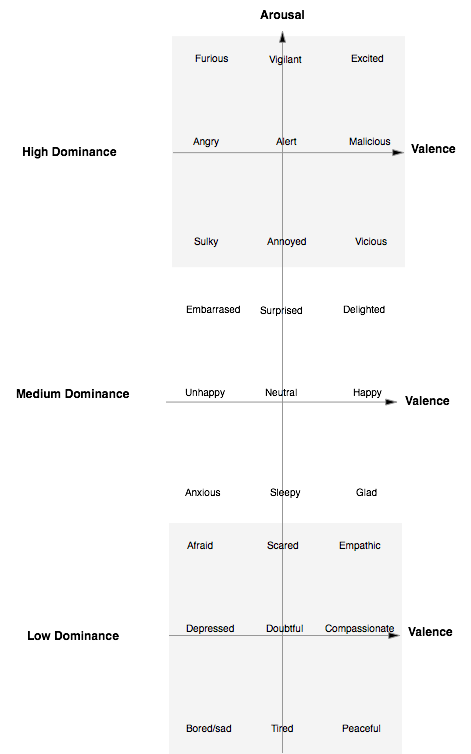
\includegraphics[height=5in]{VAD.png}}
\begin{minipage}{0.6\textwidth}
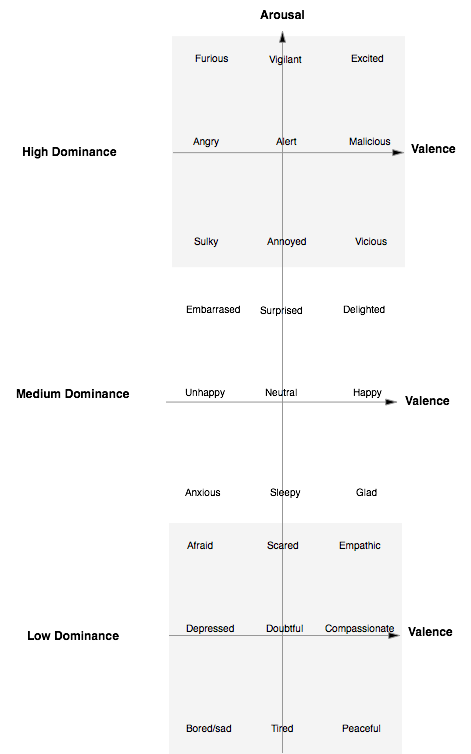
\includegraphics[width=\textwidth]{VAD.png}
\end{minipage}\hfill%
\begin{minipage}{0.35\textwidth}\raggedright
The VAD model illustrates how valence, arousal and dominance values map to identifiable emotions. Valence, arousal and dominance can each have a value of low, medium or high. This allows the agents to have a total of 27 distinct emotional states.
The valence and arousal levels of each agent are affected by the actions of other agents. For example, a character being chased around the stage by Punch will see their valence level drop while their arousal increases. According to Russell's circumplex model of emotion~\cite{russell1980circumplex}, this would result in them becoming \emph{afraid\/} (if their dominance level is low).
\medskip

An agent's emotional state affects its ability to fulfil its institutional obligations. An agent that is \emph{furious\/} might have no problem carrying out an obligation that requires them to kill another agent. If that same agent is \emph{happy\/} or \emph{depressed}, however, they might not have the appropriate motivation to perform such a violent action.
% \rule{\textwidth}{2cm}
\end{minipage}
\caption{VAD emotional values (figure adapted from Ahn et al.)~\cite{ahn2012nvc}} \label{fig:vad}
\end{figure}
In order to make the agents acting out the Punch and Judy show more believable, we apply an emotional model to affect their actions and decisions. For this, we use the valence-arousal (circumplex) model first described by Russell~\cite{russell1980circumplex}.  To give each character its own distinct personality, we extend this model with an extra dimension: dominance, as used by Ahn et al.~\cite{ahn2012nvc} in their model for conversational virtual humans. This dominance level is affected by the reactions of the audience to the agents' actions. For example, Judy may become more dominant as her suggestions to hit Punch with a stick are cheered on by the audience, emboldening her into acting out her impulses.  A detailed description appears in the text in Figure~\ref{fig:vad}.

%% Figure~\ref{fig:vad} shows how valence, arousal and dominance values map to identifiable emotions. Valence, arousal and dominance can each have a value of low, medium or high. This allows the agents to have a total of 27 distinct emotional states.
%% The valence and arousal levels of each agent are affected by the actions of other agents. For example, a character being chased around the stage by Punch will see their valence level drop while their arousal increases. According to Russell's circumplex model of emotion~\cite{russell1980circumplex}, this would result in them becoming \emph{afraid\/} (if their dominance level is low).

%% An agent's emotional state affects its ability to fulfil its institutional obligations. An agent that is \emph{furious\/} might have no problem carrying out an obligation that requires them to kill another agent. If that same agent is \emph{happy\/} or \emph{depressed}, however, they might not have the appropriate motivation to perform such a violent action.

It is important to note that the emotional model is part of the agent belief state, and not held in the institution. We want to explore how the characters of the story might be able to choose actions based on their emotional state. While the institution could theoretically calculate the emotional state for each agent in turn and dictate this to them along with the norms of the narrative, it makes sense to decouple this feature from the narrative institution in order to separate the characters from the events of the story. %\jnote{review this paragraph}

Agents' emotional states change according to their interactions with the audience. This is unrelated to what is happening in the narrative, and so this underscores the decision not to include any emotional modelling in the institution. Also, we want the agents to have some degree of freedom within the narrative world. They should be allowed to determine their emotions themselves, so that in extreme emotional states they can perform `irrational' or `extreme' actions that may not necessarily fit into the narrative.

\subsection{VAD emotions in Jason}
Emotions are implemented as beliefs inside an agent. An agent believes it has a certain level of valence, arousal and dominance, and it works out its emotional state based on a combination of these three factors. When the audience cheers or boos them, this changes the belief holding the relevant emotional variable, and their emotional state as a whole is recalculated.

Valence, arousal and dominance values can take values of -1 (low), 0 (medium) or 1 (high). Listing~\ref{lst:emotions} shows the emotional belief rules for an agent with medium dominance (a dominance level of 0). Note that an agent maintains beliefs about both its current emotion label (such as sleepy or happy) and the separate valence, arousal and dominance values at the same time.  Similar sets of rules handle the belief emotion for the other dominance levels.  %We address the matter of how external stimuli affect dominance in section~\ref{sec:norms as percepts}.\jnote{still needs doing}

Every time an emotional variable (valence, arousal, or dominance) changes, an agent's emotion is changed according to the rules in listing~\ref{lst:emotions}. While an agent's valence, arousal and dominance belief values affect the way it makes decisions internally, the results of combinations of these values (sleepy, happy, etc) are broadcast as external actions. The reason for this is that an agent's emotional state may affect the way in which the character is animated: changing the speed at which they move or turning their smile into a frown, for example. For this reason, whenever an emotional change takes place, the new emotion is published as an external action of the agent so that observing entities may perceive it. The Bath sensor framework described in section~\ref{sec:arch} provides the means for this evidence of the agent's internal state change to be received by the animation system and reflected accordingly in the display.

\begin{lstlisting}[float=!t,caption={Emotional rules for a character with medium dominance},label=lst:emotions,escapechar=\%,basicstyle=\scriptsize\ttfamily]
emotion(sleepy) :- valence(0) & arousal(-1) & dominance(0).
emotion(neutral) :- valence(0) & arousal(0) & dominance(0).
emotion(surprised) :- valence(0) & arousal(1) & dominance(0).
emotion(anxious) :- valence(-1) & arousal(-1) & dominance(0).
emotion(unhappy) :- valence(-1) & arousal(0) & dominance(0).
emotion(embarrassed) :- valence(-1) & arousal(1) & dominance(0).
emotion(glad) :- valence(1) & arousal(-1) & dominance(0).
emotion(happy) :- valence(1) & arousal(0) & dominance(0).
emotion(delighted) :- valence(1) & arousal(1) & dominance(0).
\end{lstlisting}

\begin{lstlisting}[float=!t,caption={AgentSpeak rules for changing an agent's emotional values from audience responses},label=lst:response,basicstyle=\scriptsize\ttfamily]
+!changeMood
  <- ?emotion(Z);
     emotion(Z).
+response(_, boo) : asking
  <- -+valence(-1);
     -+dominance(-1);
     !changeMood.
+response(_, cheer) : asking
  <- -+valence(1);
     -+dominance(1);
     !changeMood.
\end{lstlisting}

Listing~\ref{lst:response} shows the AgentSpeak rules describing how an agent's
valence and dominance levels are changed by the audience cheering or booing
their actions. These AgentSpeak plans describe what the agent should do in
response to a goal addition (denoted by a $\texttt{+!}$ at the start of the plan
name) or a belief addition (prefixed by a simple $\texttt{+}$). In the case of
Listing~\ref{lst:response}, the $\texttt{+!changeMood}$ plan updates the agent's
emotional state based on its valence-arousal-dominance values and broadcasts the
result as an external action. The $\texttt{+response}$ plans raise or lower an agent's valence and dominance levels depending on whether the agent perceives a ``boo'' or ``cheer'' response from the audience.

An agent announces what they intend to do, then waits three seconds. During this time, they have the belief that they are `asking' the audience, and listen for a response. A boo reduces an agent's valence and dominance, while a cheer raises them. For each response, the \texttt{changeMood} goal is triggered, which looks up and broadcasts the agent's emotional state to the other agents and environment.

\section{Agent decision making} \label{sec:decisions}
The agents choose which goals to pursue according to three factors: their permitted actions, their obliged actions and their emotional state. Though obliged actions are given priority, and while agents' decisions are generally constrained by their permitted actions, an agent's emotional state has the final say in its decisions. In this way, an agent will follow the social norms of the narrative, but only according to their own mood.

\paragraph{Agent goals and plans}
% \subsection{Agent goals and plans}
The agents are implemented using a belief-desire-intention (BDI) psychological model using the Jason platform ~\cite{bordini2007programming}. An agent's knowledge about the state of their world and themselves are stored as \emph{beliefs}, with new information coming in from the environment getting added to their belief base as \emph{percepts}, which are ephemeral and only last for one reasoning cycle of an agent.

Agents are created with goals and plan libraries. Any goal that an agent is set on carrying out at any point is an \emph{intention}, whereas a goal that an agent has but is not yet pursuing is a \emph{desire}. Plan libraries describe the steps agents need to take in order to achieve goals, as well as how to react to changes in agents' environments.

\paragraph{Norms as percepts}\label{sec:norms as percepts}
% \subsection{Norms as percepts}\label{sec:norms as percepts}
When an event occurs, it is added to the event timeline, which is used to query the ASP (Answer Set Programming) solver to obtain the set of norms that hold after the new event has occurred. The new permissions and obligations are then added to each agent as \emph{percepts}. Each time this happens, the set of permitted and obliged actions that an agent sees is changed to be only those that apply at that instant in time, with the previous norms being discarded.

Agents choose between permitted and obliged actions based on their emotional state at the point of decision making. Obliged actions are given a higher priority over permitted ones for most of the emotional states that an agent can be in, though not always. If an agent is in a sulky mood, for example, they may decide to ignore what they are obliged to do by the narrative, even though they know there will be consequences.

For example, in the scene where Joey gives the sausages to Punch, Punch may see that he has permission to eat the sausages, drop them, fight the crocodile, run away (leave the stage) or shout for help at the crocodile or audience. His obligation for the scene, in accordance with the Punch and Judy narrative world, is to either eat the sausages himself, or let the crocodile have them. This ends Propp's \emph{interdiction\/} story function with a \emph{violation\/} function. Note that his obligation in this case is not to guard the sausages as asked to by Joey. While Joey's entrusting of the sausages is certainly an obligation in itself, Punch's main obligations are to the narrative. Lesser obligations towards characters in the story can be implemented as having a lower prority than those of the story itself.

Similarly, at times of extreme emotion, an agent may decide to disregard their set of permitted actions entirely, instead acting out their innermost desires. For example, an angry Punch might decide to just attack Joey instead of agreeing to look after the sausages, or he might just decide to give up and leave if he is depressed. The key point is that the norms act as the will of the \emph{narrative}, guiding the story forward, rather than a strict set of rules that the agents must follow at all costs.

\emph{Violation events\/} add percepts to the agents telling them that they are in violation of the narrative norms. Once an agent receives such a percept, an emotional variable is changed. Typically, their dominance will decrease. The reasoning behind this is that if agents are unwilling to participate in the story, they should have less influence in its course of events.

\section{Architecture}\label{sec:arch}

\paragraph{Multi-Agent System} \label{sec:inst}
% \subsection{Multi-Agent System} \label{sec:inst}
We use the JASON framework for belief-desire-intention (BDI) agents~\cite{bordini2007programming}, programming our agents in the AgentSpeak language.
The VAD emotional model is represented inside each agent as a set of beliefs. Each agent has beliefs for its \emph{valence}, \emph{arousal} and \emph{dominance} levels, each of which can take the value of low, medium or high, as discussed in section~\ref{sec:emotion}. This combination of VAD values creates one of the 27 emotional states shown in figure~\ref{fig:vad}, affecting whether or not an agent breaks from its permitted or obliged behaviour.

\paragraph{Institutional Framework}
% \subsection{Institutional Framework}
% How you used instAL to model Propp
To describe our institutional model, we use InstAL~\cite{cliffe2007specifying}, a domain-specific (action) language for describing institutions that compiles to AnsProlog, a declarative programming language for Answer Set Programming (ASP). InstAL's semantics are inspired by the Situation Calculus~\cite{reiter1991frame} and the Event Calculus~\cite{kowalski1989logic}. InstAL describes how external events generate institutional events, which then initiate or terminate fluents that hold at certain points in time. These fluents can include the permissions and obligations that describe what an agent is permitted or obliged to do when, as described in section~\ref{sec:institutional model}.
For example, if an agent with the role of \emph{dispatcher\/} leaves the stage,
it generates the Propp \emph{absentation\/} move in the institution, but only if
the \emph{interdiction} function is active (i.e., the
\emph{activeFunction(interdiction)} fluent holds): %\mnote{Added \emph{activeFunction} explanation}
\begin{lstlisting}[basicstyle=\scriptsize\ttfamily]
leaveStage(X) generates intAbsentation(X)
   if role(X, dispatcher), activeFunction(interdiction);
\end{lstlisting}
% \vspace{-1cm}
which generates the following AnsProlog code:\\
\begin{minipage}{0.6\textwidth}
\begin{lstlisting}[basicstyle=\scriptsize\ttfamily,escapechar=\%]
occurred(intAbsentation(X),pj,I) :-%\mylabel{t1}%
   occurred(leaveStage(X),pj,I),%\mylabel{t2}%
   holdsat(pow(pj,intAbsentation(X)),pj,I),%\mylabel{t3}%
   holdsat(role(X,donor),pj,I),%\mylabel{t4}%
   holdsat(activeFunction(interdiction),pj,I), %\mylabel{t5}%
   agent(X), inst(pj), instant(I).%\mylabel{t6}%
\end{lstlisting}
\end{minipage}\hspace{0.08\textwidth}%\hfill
\begin{minipage}{0.3\textwidth}\scriptsize
\myref{t1}{s1}{The internal \emph{absentation} event occurs if the following conditions are met:}
\myref{t2}{s2}{$\bullet X$ leaves the stage}
\myref{t3}{s3}{$\bullet X$ has the power to leave the stage}
\myref{t4}{s4}{$\bullet X$ has the role of donor}
\myref{t5}{s5}{$\bullet$ the \emph{interdiction} function is active}
\myref{t6}{s6}{$\bullet X$ is an agent, pj is an institution, $I$ is an instant}
\end{minipage}\\
The \emph{absentation\/} institutional event gives the crocodile permission to enter the stage if there are any sausages on the stage. It also terminates the permission of the absented agent to leave the stage, as they have already done so:\\
\begin{minipage}{0.6\textwidth}
\begin{lstlisting}[basicstyle=\scriptsize\ttfamily,escapechar=\%]
intAbsentation(X) initiates perm(enterStage(croc)) if objStage(sausages);%\mylabel{t1}%
intAbsentation(X) terminates onStage(X), perm(leaveStage(X));%\mylabel{t2}%
\end{lstlisting}
\end{minipage}\hspace{0.08\textwidth}%\hfill
\begin{minipage}{0.3\textwidth}\scriptsize
  \myref{t1}{s1}{The \emph{absentation} function gives the crocodile permission to enter the stage if the sausages are on stage}
  \myref{t2}{s2}{The \emph{absentation} function means that once X leaves the stage, they are no longer on stage}
\end{minipage}\\
which generates the following:\\
\begin{minipage}{0.6\textwidth}
\begin{lstlisting}[basicstyle=\scriptsize\ttfamily,escapechar=\%]
initiated(perm(enterStage(croc)),pj,I) :-%\mylabel{t1}%
   occurred(intAbsentation(X),pj,I),%\mylabel{t2}%
   holdsat(live(pj),pj,I), inst(pj),%\mylabel{t3}%
   holdsat(objStage(sausages),pj,I),%\mylabel{t4}%
   agent(X), inst(pj), instant(I).%\mylabel{t5}%
\end{lstlisting}
\end{minipage}\hspace{0.08\textwidth}%\hfill
\begin{minipage}{0.3\textwidth}\scriptsize
\myref{t1}{s1}{The crocodile gets permission to enter the stage if the following
  conditions are met:}
\myref{t2}{s2}{$\bullet$ the \emph{absentation} function event has occured}
\myref{t3}{s3}{$\bullet$ the pj institution is running}
\myref{t4}{s4}{$\bullet$ the sausages are on stage}
% \myref{t5}{s5}{$\bullet X$ is an agent, pj is an institution, $I$ is an instant}
\end{minipage}\\
%% \begin{comment}
%% If the ``defeat'' institutional event occurs (as a result of a struggle between
%% two agents), it initiates a fluent signifying that that agent is dead, along
%% with an obligation for the agent to leave the stage. If they don't leave the
%% stage, then they are in violation of the scene, and an appropriate violation
%% event is triggered. Also note that the fluent and obligation event are only
%% initiated \emph{if} the agent is playing the role of a victim:
%% \begin{lstlisting}[basicstyle=\scriptsize\ttfamily]
%% intDefeat(X, Y) initiates dead(Y), obl(leaveStage(Y), deadline, vioScene(Y)) if role(Y, victim);
%% \end{lstlisting}
%% \end{comment}
\begin{figure}[!t]
\begin{minipage}{0.6\textwidth}
\begin{lstlisting}[caption={Encoding of Propp's \emph{absentation\/} function},basicstyle=\scriptsize\ttfamily,label=lst:absentation,escapechar=\%]
intAbsentation(X) initiates activeFunction(absentation);%\mylabel{t0}%
intAbsentation(X) initiates perm(harm(Y, Z)) if role(Y, villain), objStage(Z), onStage(Y), activeFunction(interdiction);%\mylabel{t1}%
intAbsentation(X) initiates perm(harm(Y, Z)) if role(Y, ambusher), objStage(Z), onStage(Y), activeFunction(interdiction);%\mylabel{t2}%
intAbsentation(X) initiates perm(enterStage(X)), activeFunction(absentation);%\mylabel{t3}%
intAbsentation(X) initiates perm(enterStage(croc)) if objStage(sausages);%\mylabel{t4}% 
intAbsentation(X) terminates onStage(X), perm(leaveStage(X));%\mylabel{t5}%
\end{lstlisting}
\end{minipage}\hspace{0.08\textwidth}%\hfill
\begin{minipage}{0.3\textwidth}\scriptsize
  \myref{t0}{s0}{The \emph{activeFunction(absentation)} function holds after any
    \emph{intAbsentation} institutional event, indicating that that Propp
    function is currently underway}
  \myref{t1}{s1}{The \emph{absentation} function gives the villain permission to harm
    an object, if both are on stage and the \emph{interdiction} function is active}
  \myref{t2}{s2}{Same as above, but for \emph{ambusher} role}
  \myref{t3}{s3}{The absented character has permission the re-enter the stage at any point during the \emph{absentation} function}
  \myref{t4}{s4}{The crocodile has permission to enter the stage if the sausages are on stage}
  \myref{t5}{s5}{The \emph{absentation} function means that the absented character is no longer on stage, and cannot leave the stage (as they have already done so)}
\end{minipage}
\end{figure}
By combining statements such as the above, we can build a complete description
of the sausages scene in terms of agent norms, such as the Propp
\emph{absentation} function, shown in Listing~\ref{lst:absentation}. InstAL rules like those shown above and in Listing~\ref{lst:absentation} are compiled into AnsProlog, then we use the \emph{clingo} answer set solver~\cite{gebser2011potassco} to ground the program, and `solve' queries by finding all permissions and obligations that apply to any agents, given a sequence of events as the query input. The agents' percepts are then updated with their permitted and obliged actions from that time instant onwards.  Thus, the institutional model acts as a social narrative sensor, interpreting actors' actions in the context of the combination of the concrete narrative and the abstract story moves which detach (instantiate) the norms that guide the actors in the direction of the conclusion of the story arc.

A query is simply a list of external events in chronological order, also called
a \emph{trace}. A possible trace describing the actions of agents acting out the
\emph{sausages} is described in Listing~\ref{lst:trace}. The `pj' in the trace
is the name of the institution that observes the events, while the
number is the enumeration of events in the sequence.

\begin{figure}[!t]
\begin{minipage}{0.6\textwidth}
% \newsavebox{\lstasp}
% \begin{lrbox}{\lstasp}
\begin{lstlisting}[caption={Possible full trace for sausages scene},label=lst:trace,basicstyle=\scriptsize\ttfamily,escapechar=\%]
observed(startShow,pj,0). %\mylabel{t1}%
observed(startScene(sausages),pj,1). %\mylabel{t2}%
observed(enterStage(punch),pj,2). %\mylabel{t3}%
observed(enterStage(joey),pj,3). %\mylabel{t4}%
observed(say(joey, give),pj,4). %\mylabel{t5}%
observed(say(joey,  protect),pj,5). %\mylabel{t6}%
observed(give(joey,punch,sausages),pj,6). %\mylabel{t7}%
observed(leaveStage(joey),pj,7). %\mylabel{t8}%
observed(say(punch, harm),pj,8). %\mylabel{t9}%
observed(enterStage(croc),pj,9). %\mylabel{t10}%
observed(take(croc, sausages),pj,10). %\mylabel{t11}%
observed(eat(croc, sausages),pj,11). %\mylabel{t12}%
observed(leaveStage(croc),pj,12). %\mylabel{t13}%
observed(enterStage(joey),pj,13). %\mylabel{t14}%
observed(hit(joey, punch),pj,14). %\mylabel{t15}%
observed(leaveStage(joey),pj,15). %\mylabel{t16}%
observed(leaveStage(punch),pj,16). %\mylabel{t17}%
observed(startScene(end),pj,17). %\mylabel{t18}%
\end{lstlisting}
\end{minipage}\hspace{0.08\textwidth}%\hfill
\begin{minipage}{0.3\textwidth}\scriptsize
  \myref{t1}{s1}{The show has started}
  \myref{t2}{s2}{The sausages scene has started}
  \myref{t3}{s3}{Punch has entered the stage}
  \myref{t4}{s4}{Joey has entered the stage}
  \myref{t5}{s5}{Joey says he will give Punch the sausages}
  \myref{t6}{s6}{Joey tells Punch to protect the sausages}
  \myref{t7}{s7}{Joey gives the sausages to Punch}
  \myref{t8}{s8}{Joey leaves the stage}
  \myref{t9}{s9}{Punch says he will eat the sausages}
  \myref{t10}{s10}{The crocodile enters the stage}
  \myref{t11}{s11}{The crocodile takes the sausages}
  \myref{t12}{s12}{The crocodile eats the sausages}
  \myref{t13}{s13}{The crocodile leaves the stage}
  \myref{t14}{s14}{Joey enters the stage}
  \myref{t15}{s15}{Joey hits Punch}
  \myref{t16}{s16}{Joey leaves the stage}
  \myref{t17}{s17}{Punch leaves the stage}
  \myref{t18}{s18}{The scene ends}
\end{minipage}
\end{figure}

Each \emph{observed} event triggers a corresponding \emph{occurs} event inside the
institution, as determined by the generates relation. Listing~\ref{lst:asp}
shows an extract from an answer set output for the trace queried against the ASP
description of the sausages scenario, for events~5 to~7 of the scene. Starting with an initial set of fluents that hold at instant~5,
only fluents that have been initiated and not terminated hold at the next
instant. For ease of reading, the listing only shows roles that hold at
certain instants when they have some effect on the scene, although in practice, all role fluents hold throughout the scene. Figure~\ref{fig:tracevis} shows a visualisation of the answer set for the trace in listing~\ref{lst:trace}.

\begin{figure}[!t]
\begin{minipage}{0.65\textwidth}
%% \newsavebox{\lstasp}
%% \begin{lrbox}{\lstasp}
\begin{lstlisting}[caption={Sausages scene using ASP},label=lst:asp,basicstyle=\scriptsize\ttfamily,label=lst:asp,escapechar=\%]
holdsat(perm(say(donor, protect),pj,5).%\mylabel{t1}%
holdsat(role(joey, donor),pj,5).%\mylabel{t2}%
occurred(say(joey, protect),pj,5).%\mylabel{t3}%

initiated(activeFunction(interdiction),pj,6).%\mylabel{t4}%
initiated(perm(give(donor, villain, object)),pj,6).%\mylabel{t5}%
terminated(perm(say(donor, protect)),pj,6).%\mylabel{t6}%
holdsat(perm(give(donor, villain, object)),pj,6).%\mylabel{t7}%
holdsat(activeFunction(interdiction),pj,6).%\mylabel{t8}%
holdsat(role(joey, donor),pj,6).%\mylabel{t9}%
holdsat(role(punch, villain),pj,6).%\mylabel{t10}%
holdsat(object(sausages),pj,6).%\mylabel{t11}%
occurred(give(joey, punch, sausages),pj,6).%\mylabel{t12}%

initiated(activeFunction(absentation),pj,7).%\mylabel{t13}%
initiated(perm(leavestage(donor)),pj,7).%\mylabel{t14}%
terminated(perm(give(donor, villain, object)),pj,7).%\mylabel{t15}%
holdsat(activeFunction(interdiction),pj,7).%\mylabel{t16}%
holdsat(activeFunction(absentation),pj,7).%\mylabel{t17}%
holdsat(role(joey, donor),pj,7).%\mylabel{t18}%
holdsat(perm(leavestage(donor)),pj,7).%\mylabel{t19}%
\end{lstlisting}
\end{minipage}\hspace{0.03\textwidth}%\hfill
% \end{lrbox}
% \noindent\usebox{\lstasp}\hfill
\begin{minipage}{0.3\textwidth}\scriptsize
  \myref{t1}{s1}{The donor role can tell someone to protect an object at instant 5}
  \myref{t2}{s2}{Joey is the donor at instant 5}
  \myref{t3}{s3}{Joey tells another character to protect an object at instant 5}
  \myref{t4}{s4}{The \emph{interdiction} function becomes active at instant 6}
  \myref{t5}{s5}{The donor has permission to give an object to the villain at instant 6}
  \myref{t6}{s6}{The donor can no longer tell anyone to protect an object at instant 6}
  \myref{t7}{s7}{The donor can give an object to the villain at instant 6}
  \myref{t8}{s8}{The \emph{interdiction} function is active at instant 6}
  \myref{t9}{s9}{Joey is the donor at instant 6}
  \myref{t10}{s10}{Punch is the villain at instant 6}
  \myref{t11}{s11}{Sausages are an object at instant 6}
  \myref{t12}{s12}{Joey gives the sausages to Punch at instant 6}
  \myref{t13}{s13}{The \emph{absentation} function becomes active at instant 7}
  \myref{t14}{s14}{The donor can leave the stage at instant 7}
  \myref{t15}{s15}{The donor can give an object to the villain at instant 7}
  \myref{t16}{s16}{The \emph{interdiction} function is active at instant 7}
  \myref{t17}{s17}{The \emph{absentation} function is active at instant 7}
  \myref{t18}{s18}{Joey is the donor at instant 7}
  \myref{t19}{s19}{The donor can leave the stage at instant 7}
\end{minipage}
\end{figure}

% \begin{figure}[!t]
% 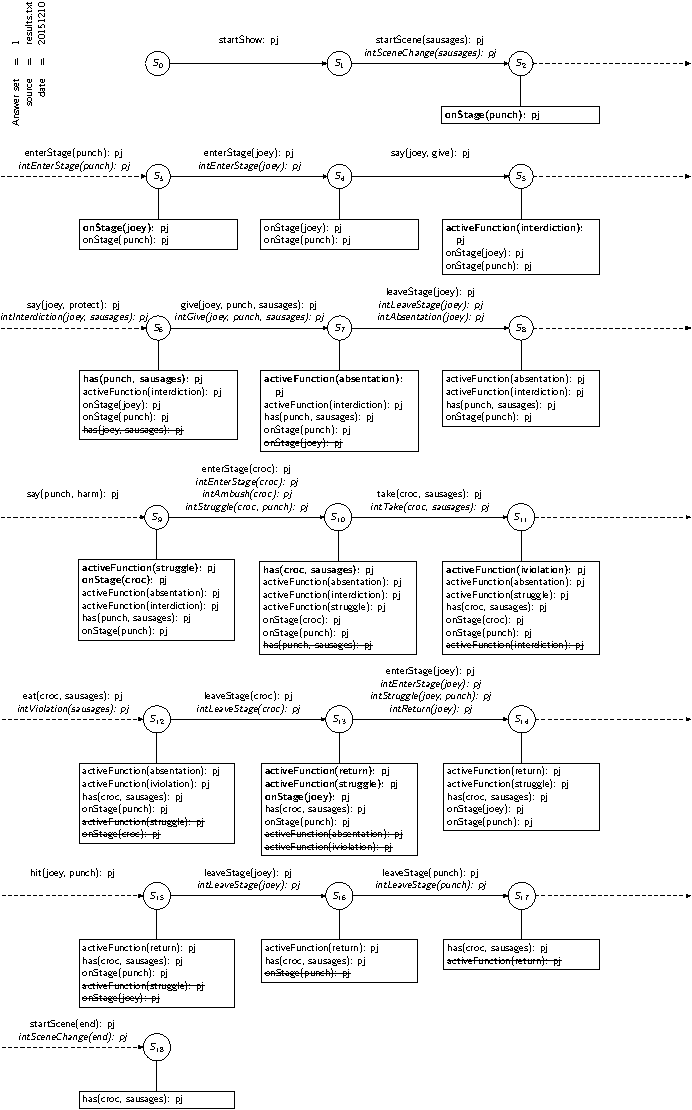
\includegraphics[width=1.3\linewidth]{trace.pdf}
% \caption{Visualised trace of the sausages scene} \label{fig:vis}
% \end{figure}

\begin{figure}[!p]
%     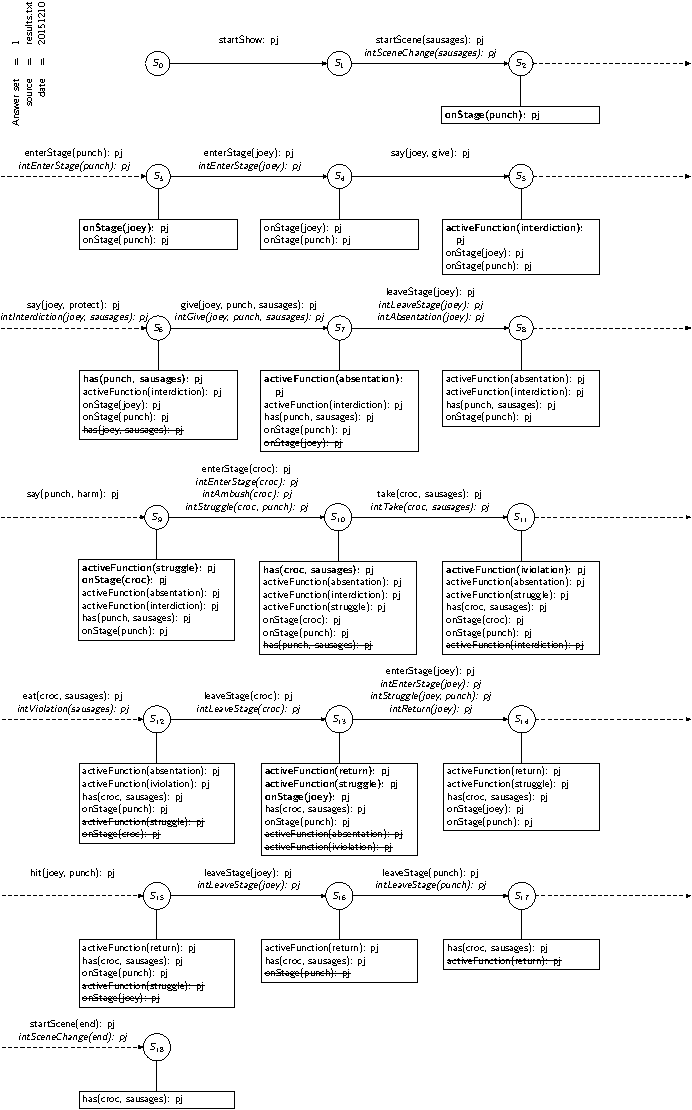
\includegraphics[width=\linewidth]{trace.pdf}
    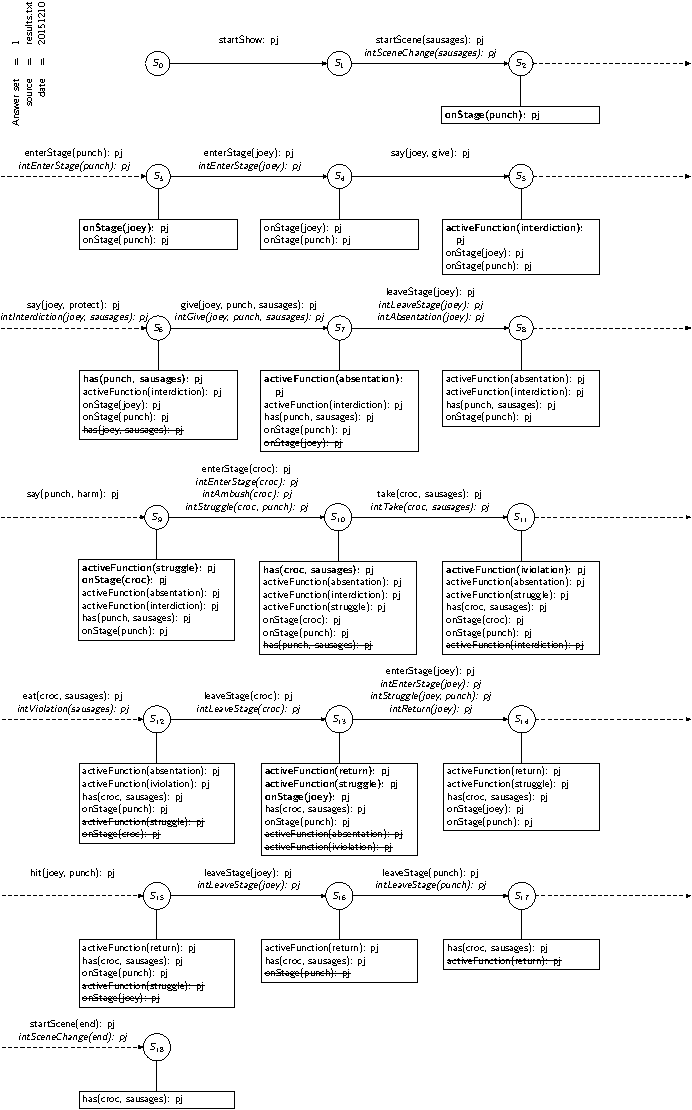
\includegraphics[height=0.95\textheight]{trace.pdf}
    \caption{Trace visualisation} \label{fig:tracevis}
\end{figure}

% 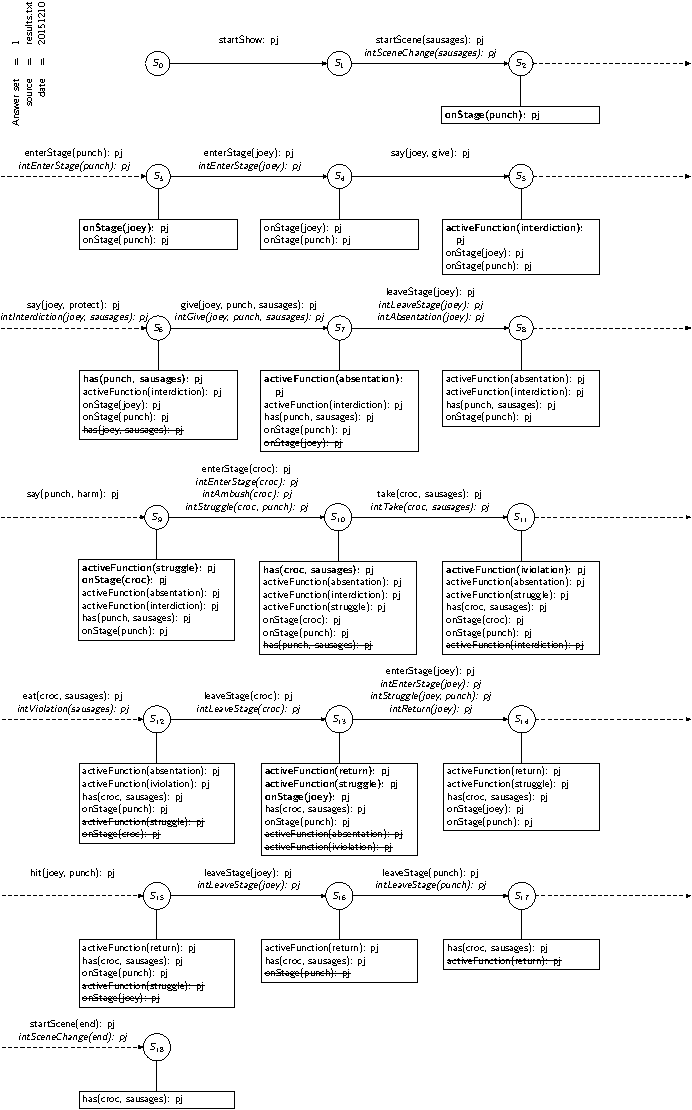
\includepdf{trace.pdf}

%\lstinputlisting[language=prolog, firstline=74, lastline=74]{pj_model.ial}

%\begin{lstlisting}[language=prolog, frame=single]  % Start your code-block
%enterStage(X) generates intReturn(X, Z) if role(X, dispatcher), role(Y, villain), onStage(Y);
%\end{lstlisting}

\begin{figure}[!t]
% \includegraphics[height=3in]{arch1.png}
% \begin{minipage}{0.58\textwidth}
% \includegraphics[width=\textwidth]{arch1.png}
% \end{minipage}\hfill
% \begin{minipage}{0.38\textwidth}\raggedright
% \end{minipage}
% \caption{System architecture} \label{fig:arch}
% % \end{figure}
% % \begin{figure}[!t]
% \medskip
\begin{minipage}{0.56\textwidth}
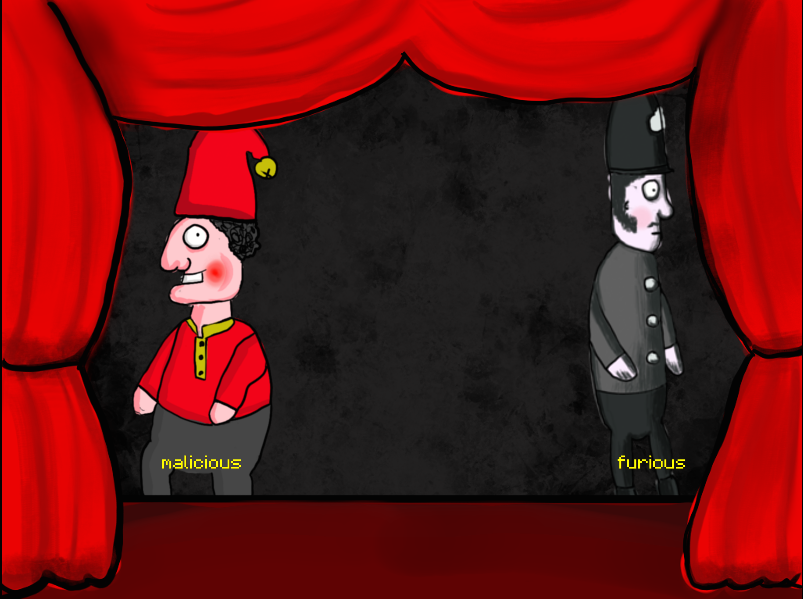
\includegraphics[width=\textwidth]{punchjudy.png}
\end{minipage}\hfill%
% 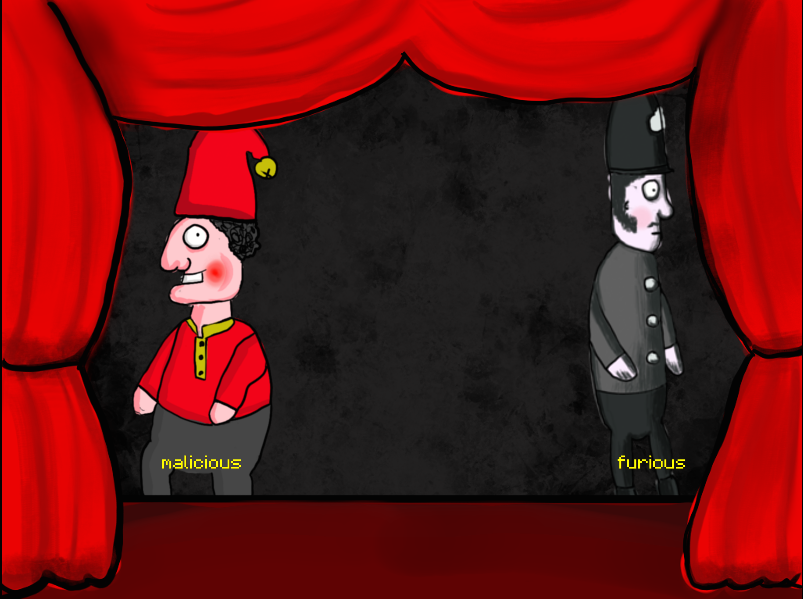
\includegraphics[height=2in]{punchjudy.png}
\begin{minipage}{0.4\textwidth}
% The animation engine that shows the visual output of the agents actions is written in Javascript and the Phaser game framework. It runs entirely in a browser, and communicates with BSF using the Strophe XMPP library.
The animation engine that shows the visual output of the agents actions is written in Javascript and the Phaser game framework. It runs entirely in a browser, and communicates with BSF using the Strophe XMPP library.

If the user allows the program access to their microphone, they can cheer or boo the actions of the agents by shouting into the microphone. Otherwise, they can simulate these actions by clicking on `cheer' or `boo' buttons at the bottom of the screen.
\end{minipage}
\caption{A screenshot of the Punch and Judy show} \label{fig:pjshow}
\end{figure}

\paragraph{Bath Sensor Framework} The components communicate using the Bath Sensor Framework
(BSF)~\cite{lee2013decoupling}, through publish / subscribe-style communication between distributed software components, in this case connecting intelligent agents with their virtual environments. It currently uses the XMPP publish/subscribe protocol for communication between agents, environment and other software components. Each agent subscribes to receive notifications of environment changes via the appropriate topic node in the XMPP server, which relays messages between publishers and subscribers. If any environment change occurs, all subscribed agents are informed of the changes.

\begin{comment}
\paragraph{Bath Sensor Framework} \label{sec:bsf}
%\subsection{Bath Sensor Framework} \label{sec:bsf}
% Just say it uses XMPP to glue components together
The Bath Sensor Framework (BSF)~\cite{lee2013decoupling} supports publish / subscribe-style communication between distributed software components, in this case connecting intelligent agents with their virtual environments. It currently uses the XMPP publish/subscribe protocol for communication between agents, environment and other software components. Each agent subscribes to receive notifications of environment changes via the appropriate topic node in the XMPP server, which relays messages between publishers and subscribers. If any environment change occurs, all subscribed agents are informed of the changes.

An XMPP server offers two topic nodes: environment, for environment change
events and norm for agent permission and obligation change events.  All agents
(in this case, Punch, Judy, the Policeman, etc) subscribe to both topics and
publish to environment, but not to norm. The institution manager (connected to
the \emph{clingo} solver) subscribes to environment and publishes (permissions
and obligations) to norm. Environment events are passed to \emph{clingo} with
the institutional model, to generate new permissions and obligations, to
publish.  The animation engine subscribes to environment, to receive events to
animate for the puppet show. It can also publish input from the audience
(`cheers' or `boos') as events to the environment.%\mnote{Replaced arch diagram  with this description}

This approach allows agents' environments to be created using entirely different technologies and programming languages from the agents themselves. In our case, BSF is especially useful as the animation engine that acts as the agents' environment is written in Javascript and runs in the browser. This means that the clingo solver and JASON agent framework can run on another server and communicate to any connected clients using BSF and XMPP. A screen shot from the animation engine appears in Figure~\ref{fig:pjshow}. %% Figure~\ref{fig:arch} shows how BSF is used to coordinate the components of the system. An XMPP server runs two publish/subscribe nodes. One node is for events related to changes in the environment (the \emph{environment} node), the other is for changes in agents' permissions and obligations (the \emph{norm} node).


%% All agents (in this case, Punch, Judy, the Policeman, etc) subscribe to both the environment and norm nodes. They can also publish events to the environment node, but not the norm node. Only the institution manager (connected to the \emph{clingo} solver) can publish permissions and obligations to the norm node. This manager (labelled in figure~\ref{fig:arch} as \emph{institution manager}) subscribes to the environment node of the XMPP server, watching it for events. These events then get passed to the \emph{clingo} solver with the institutional model, which outputs the new permissions and obligations, publishing them to the norm node.

%% The animation engine subscribes to the environment node, watching it for any events that need animating for the puppet show. In addition, it can publish input from the audience (`cheers' or `boos') as events to the same node.

%\subsection{Animation} \label{sec:anim}
%% % CoffeeScript, Phaser, running in browser
The animation engine that shows the visual output of the agents actions is written in Javascript and the Phaser game framework. It runs entirely in a browser, and communicates with BSF using the Strophe XMPP library.

If the user allows the program access to their microphone, they can cheer or boo the actions of the agents by shouting into the microphone. Otherwise, they can simulate these actions by clicking on `cheer' or `boo' buttons at the bottom of the screen. In situations where a large audience is cheering or booing at the show, ambiguous audience input can be overcome by having a person click these buttons according to whichever response they think to be more popular.

\end{comment}

\paragraph{Audience Interaction} \label{sec:demo}
% Explain what will happen
The puppet show is designed to be run in front of either a single user's computer, or on a large display in front of an audience. The user/audience is instructed to cheer or boo the actions of the characters of the show, which will be picked up by a microphone and `heard' by the agents. This will then affect the emotional state of the agents and change the actions they make in the show. Their actions are constrained by the set of `Punch and Judy' world norms as described in the institutional model.

There are many different ways in which the audience's responses can affect the outcomes of the show. If the audience craves a more `traditional' Punch and Judy experience, then they can cheer Punch into beating and killing all of his adversaries (including his wife, Judy). Alternatively, a more mischievous audience could goad Judy into killing Punch and then taking over his role as sadist and killer for the rest of the show. The narrative outcomes are dependent on how the audience responds to the action, yet still conform to the rules of the Punch and Judy story world.

\section{Related Work}
Many approaches exist for creating interactive drama using agents as characters.
Carnegie Mellon's OZ project~\cite{DBLP:books/sp/wooldridgeV99/Mateas99} is one of the first
major research efforts to use agents for
interactive narrative. A dramatic structure is given to the narrative by means
of a \emph{drama manager}, which is able to see all of the actions occurring in
the story world and can change anything in order to create a better experience
for the user. While a drama manager rigidly enforces
agents to conform to the expectations of a story, our approach differs in that
it regulates the agents, allowing them some degree of agency. This allows the agents to break from the set of actions suggested by a story function. If multiple institutions present alternative sets of story functions to the agents as norms, then this means that the agents would have some freedom to change the course of the story, while the institutions ensure a coherent narrative.

Ideas from the OZ project were later developed into what became Mateas's and Stern's \emph{Fa\c{c}ade}, where players interact with the characters of the story through natural language. In this game, the player attends the party of a young couple (Grace and Trip) celebrating their wedding anniversary. As the course of events unfold however, the player learns that all is not as happy as it seems.

In Fa\c{c}ade, the smallest unit of narrative action is called a \emph{story
  beat}, taken from McKee's book on authorial style for
screenwriters~\cite{mckee1997substance}. The simulation constantly monitors what
the user is doing and how it may lead from the current story beat to another. Story beats
have preconditions and effects on the state of the narrative, so it is the drama
manager's job to work out when it makes sense to initiate a certain beat. They
can be thought as analogous to Propp's story functions, but in contrast to the
work presented here, operate at a lower level of
abstraction, describing specific agent goals and the steps needed to achieve them. Our use of norms allows abstract story components to be written without the need to write agent goals for story events. Instead, their existing plans are governed by institutions, and guided towards taking actions to fulfil the story components.

Riedl and Young make much use of agents and planners in their work on
interactive narrative. Addressing the problem of balancing character
believability with plot coherence, they present a planner-based solution for
story generation~\cite{riedl2004intent}. Their planner is described as an
`intent-driven partial order causal link' planner, planning actions for agents
in a multi-agent system based on causality and intention. In this case,
\emph{intention} refers to a component of agents based on the Belief Desire
Intention (BDI) framework. Their planner observes the actions of the agents in
the system and infers their intentions. While their planners have the
flexibility to revise their plans based on user interactions, they still rely on
an author creating all possible alternative plans that allow the agents to act
out a story. Again, our use of institutions allows for story authoring on a
higher level, where an author need not be concerned with writing plans.

\section{Conclusions and Future Work}

With our approach to interactive narrative generation, we regulate the rules of
the story domain using an institutional model. This model describes what each
agent is permitted and obliged to do at any point in the story. This approach
alone would be too rigid, however. The audience's interactions (cheering or
booing) may alter the course of the narrative, but the agents would still have
blindly to follow a pre-determined set of paths. By giving our agents emotional
models that change their willingness to follow the narrative, a degree of
unpredictability enters each performance, giving the impression that the agents
are indeed characters capable of free will. The VAD emotional model is
essentially reactive and quite simplistic.  A more deeply-rooted emotional
response, perhaps better aligned with BDI, could be achieved, based on the
appraisal theory of emotion. We also note that Propp's formalism is very specific to Russian folktales and could be replaced with something more general, such as Lehnert's story functions~\cite{lehnert1981plot}. Cavazza et al.~\cite{cavazza2009iris} suggest the use of Linear Logic as a promising possibility for narrative formalisation, with Martens et al.~\cite{martens2013linear} exploring its use further.

In our current approach, we describe the use of institutions for the modelling of narrative. There are two major unconsidered aspects in the current implementation, namely how to manage multiple scenes and how to preserve information between scenes.

The current Propp-based method is only suitable for modelling either one scene per institution or the complete narrative as a fixed sequence of scenes as one institution. Either way, the order of scenes is not governed in any way, but is pre-determined, whereas to create a truly non-linear narrative, the sequence must be changeable as the simulation or game is running.  A solution would be a mechanism to coordinate multiple institutions dynamically, but still according to some higher level narrative.~\cite{DBLP:conf/atal/KingLVDJPR15} describe the use of \emph{metanorms\/} or \emph{higher-order norms\/} to enable institutions to govern other institutions, which could be applied in InstAL to create a multi-tier institution for narrative.

A second issue is how to retain information between scenes: if a set of narrative events have occurred in one scene, their consequences often need to be carried over to other scenes, which implies the transfer of fluents between institutions.~\cite{bath38667} describe a mechanism to bridge institutions, which could be used to control the flow of events and facts between institution instances.

In meeting both these requirements, a \emph{hierarchy\/} of institutions is needed to govern the narrative world: a kind of `scene director' institution to manage the flow between scene institutions, and a means to share information in order to achieve narrative consistency and persistence. Such a combination of multi-tiered and co-operating institutions offers the potential for the generation of a much richer way of regulating narrative events in a multi-agent system.  The simple proof-of-concept set out in this paper provides a first step towards developing an institutional model for narrative as well as a preliminary validation of the WIT model.


\chapter{Future Work}
\label{sec:future}



\chapter{Literature Review}
\label{cha:literature-review}

This research covers multiple fields of study such as narratology, interactive
storytelling, emotional modelling and artificial intelligence, therefore an extensive
literature review covering these fields is necessary. This section starts with a
look at the field of \emph{narratology}, or narrative theory, to gain some
insights into the themes and components that make up stories. Looking at
different formalisms that have been created for narrative and which themes and
motifs recur in stories should better inform the creation of techniques with
which to generate stories.

We also examine current approaches to interactive narrative generation,
focussing particularly on the use of planners, drama managers, social norms and
logical modelling for describing stories. Most of these implementations are
designed with multi-agent systems in mind, where the story forms a set of rules
which govern these agents. The start of this part of the literature survey also
examines non-interactive story generation through means of techniques such as
generative grammar, in order to provide a historical context for the research
that follows. 

As part of the examination of implementations of interactive narrative, this review especially focuses on agent-based systems. The section concludes with an overview of emotional models that can be used to model distinct characters using agents.

\section{Narratology}
\label{sec:narratology}
Narratology is a deep field with many sub-fields. This review examines the parts of it that might best inform the modelling of narrative by computers, as well as the construction of interactive narrative.

The first part of the overview of narratology examines research into categorising different types of narrative, both traditional and experimental.
This draws from classic narratological texts, as well as work done on
``cybertext'' and experimental narrative in the interactive age. This
examination of recent research into non-linear narratives is essential for the
construction of interactive narratives for games or simulations.

Structuralist formalisms of narrative attempt to explain how stories work by dividing them into commonly occuring themes and motifs. This is a natural fit to the modelling of narratives by computer. This overview of narratology starts with structuralism for this reason.

After the overview of structuralists' narrative models there follows a section on the use of formal logic for narrative modelling. The section ends with descriptions of other types of story components, taxonomies and ontologies used in the literature.

\subsection{Narrative Structure}
\label{sec:structure}
What is the difference between a narrative and a sequence of events? If we
recount the events that happened to us during the course of a day, would that
``count'' as a narrative? When is the retelling of events a simple listing of
facts, and when is it a story?

Narratologists from \citet{bal2009narratology} onwards refer to the
chronological ordering of events as \emph{fabula} (from the Russian фабула, ``scene''), and the retelling and
reordering of those events in a narrative as \emph{syuzhet} (сюжет, ``plot'').
In fact, Russian structuralists~\citet{propp1968morphology} and~\citet{shklovsky1991theory} were the first to use these terms in the
context of narrative, before their rediscovery by modern narrative theorists.

The concepts of \emph{fabula} and \emph{syuzhet} are key to the understanding of
narrative structure. Thanks to Aristotle's
\emph{Poetics}~\citep{halliwell1986aristotle}, we understand that a story must
have a beginning, a middle and and end. These three parts of a story describe
how the \emph{syuzhet} are organised, which can refer to its \emph{fabula}
(chronological) events in any order. For example, the beginning of a movie could
be set at the present day in the life of the protagonist, the middle could be a
flashback to an earlier time in her life, and the end could return to the events
following the start of the movie.

Though Aristotle identifies the beginning, middle and end as three key story
divisions, other theorists divide the \emph{syuzhet} of a story further. Joseph
Campbell's work \emph{The Hero with a Thousand Faces}~\citep{campbell2008hero}
describes how almost every story is a variation of the \emph{Hero's Journey}
(which Cambell also calls the \emph{monomyth}). Like Aristotle's beginning, middle and end,
the Hero's Journey has three acts: the Departure, the Initiation and the Return.
Campbell divides these acts further into seventeen distinct stages:

\paragraph{Departure}
\begin{myenumerate}
  \item The Call to Adventure
  \item Refusal of the Call
  \item Supernatural Aid
  \item Crossing the Threshold
  \item Belly of the Whale
\end{myenumerate}
\paragraph{Initiation}
\begin{myenumerate}
  \item The Road of Trials
  \item The Meeting with the Goddess
  \item Woman as Temptress
  \item Atonement with the Father
  \item Apotheosis
  \item The Ultimate Boon
\end{myenumerate}
\paragraph{Return}
\begin{myenumerate}
  \item Refusal of the Return
  \item The Magic Flight
  \item Rescue from Without
  \item The Crossing of the Return Threshold
  \item Master of Two Worlds
  \item Freedom to Live
\end{myenumerate}

In summary, the hero begins the story at home or in some otherwise familiar
setting, where she is called away on an adventure. After possibly rejecting this
call, the hero leaves home (crosses the threshold) and sets off for the land of adventure. After facing
many trials and possibly defeating an enemy, the hero returns home once again.
Having endured the many trials of the journey, our hero becomes stronger in spirit
and character.

As a classic example, consider the plot of Tolkien's \emph{The Hobbit}. At the
start of the tale, Bilbo Baggins is a comfortable but risk-averse hobbit who
refuses to leave his comfortable surroundings when Gandalf first visits to
send him on a quest. Of course, he does eventually leave home to fulfill the
quest, returning home a changed character.

Campbell argues that the \emph{monomyth} acts as a shared cultural memory of
sorts, being the universal template for the rite-of-passage tale. He says that
it is passed down as myth through many different cultures, replicating in much the same way
as genes (or memes) do and that it can be thought of as a \emph{metamyth}, or the
spiritual history of humanity.

% Polti 27
% Look at story shapes paper for inspiration
Other analysts have described several different types of commonly-seen plot.
\citet{harris1959basic} makes the case for just three types of plot, having
either a happy ending (where the protagonist is virtuous), an uphappy ending
(with a selfish protagonist) or being a tragedy (where the protagonist is struck
by fate).

\citet{booker2004seven} describes seven basic plots, where each may have either a
happy or unhappy ending:
\begin{compactitem}
  \item Overcoming the monster
  \item Rags to riches
  \item The quest
  \item Voyage and return
  \item Comedy
  \item Tragedy
  \item Rebirth
\end{compactitem}

Georges Polti famously divides narratives into the \emph{thirty-six dramatic
  situations}~\citep{polti1921thirty}, derived from his analysis of classical
Greek and both classical and contemporary French texts. Polti's thirty-six types
of plot are:

\begin{multicols}{2}
\begin{compactenum}
  \item Supplication
  \item Deliverance
  \item Crime pursued by vengeance
  \item Vengeance taken for kin upon kin
  \item Pursuit
  \item Disaster
  \item Falling prey to cruelty/misfortune
  \item Revolt
  \item Daring enterprise
  \item Abduction
  \item The enigma
  \item Obtaining
  \item Enmity of kin
  \item Rivalry of kin
  \item Murderous adultery
  \item Madness
  \item Fatal imprudence
  \item Involuntary crimes of love
  \item Slaying of kin unrecognized
  \item Self-sacrifice for an ideal
  \item Self-sacrifice for kin
  \item All sacrificed for passion
  \item Necessity of sacrificing loved ones
  \item Rivalry of superior vs. inferior
  \item Adultery
  \item Crimes of love
  \item Discovery of the dishonour of a loved one
  \item Obstacles to love
  \item An enemy loved
  \item Ambition
  \item Conflict with a god
  \item Mistaken jealousy
  \item Erroneous judgment
  \item Remorse
  \item Recovery of a lost one
  \item Loss of loved ones
\end{compactenum}
\end{multicols}

\begin{figure}[!t]
\centerline{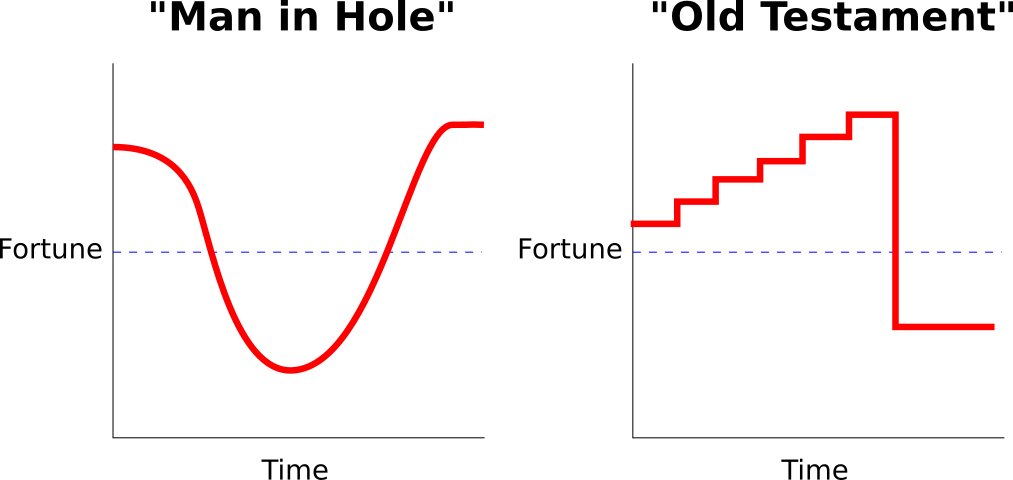
\includegraphics[height=2in]{vonnegut.png}}
\caption{Two of Kurt Vonnegut's ``Shapes of Stories''}\label{fig:vonnegut}
\end{figure}

Author Kurt Vonnegut describes several different ``shapes'' of stories in his
rejected Master's thesis~\cite{vonnegut2009palm}. He plots the events of a story
as points in a 2D space with ``Beginning-End'' (time) on the X-axis and ``Ill
Fortune-Great Fortune'' (fortune of protagonist) on the Y-axis.
Figure~\ref{fig:vonnegut} shows two examples of story shapes. In the ``Man in
Hole'' example, things start out well for the story's protagonist, but then some
misfortune falls on them. They spend much of the story overcoming challenges
before finally ending the story with a triumph. In the ``Old Testament''
example, the protagonist(s) experience gradually increasing levels of fortune,
before finally being ``cast down'' to a grave level of misfortune at the end of
the story.

All of the above categorisations describe stories as a whole, sorting narratives
into one of several different ``types'' of story. This works well for
linear narratives within traditional media, but what about experimental and
non-linear narratives? In the next section, we review the literature relating to
these less traditional types of stories.

\subsection{Types of Narrative}
% Author Kurt Vonnegut
% Look at Cybertext, etc, and try to explain how best to divide different types
% of story
The rise of the Web in the 1990s brought with it great interest in the future of narrative in cyberspace. Aarseth's work, \emph{Cybertext} \citep{aarseth1997cybertext} describes the creation of a new form of narrative, for which he coins the term \emph{ergodic literature} (from the Greek words \emph{ergon} and \emph{hodos}, meaning `work' and `path'). In this new form of narrative, some amount of work or effort is required by the reader in order to traverse the path that the story takes.

% scriptons/discourse textons/fabula (Bal 1997)
Aarseth makes a distinction between the narrative as written by the author, and the way in which it is traversed by the reader, calling the former \emph{textons} and the latter \emph{scriptons}. In ergodic literature, the \emph{scripton} is produced by the effort that the reader goes through in interpreting the \emph{texton}. In the context of a game, it is as though the game interface is a gateway that allows access to the narrative at different times. Using classical music as a metaphor, the texton can be thought of as the \emph{score}, and the scripton the \emph{performance}.

% TODO Make sure you update the intro with this
In section~\ref{sec:generative-and-interactive-narrative}, we assert that how generative a narrative is and its level of interactivity are two different variables in an experimental narrative. However, Aarseth identifies seven different methods of story traversal: \emph{dynamics, determinability, transiency, perspective, access, linking and user function}.

\textbf{Dynamics} describe whether or not the content and number of scriptons changes. In a simple, static story with branching choices (such as in a \emph{Choose your own adventure} story), both the number of textons and scriptons are fixed, since all paths have been written out beforehand. A dynamic story would still have a fixed number of textons, but the scriptons would be generated as the user traverses the path of the narrative.

\textbf{Determinability} is how deterministic the narrative is, whether or not the same interactions will result in the same scripton being produced.

\textbf{Transiency} means to what extent scriptons are produced as time flows, or whether user interactions are required to produce them.

\textbf{Perspective} is whether or not the user/reader plays a role as a character in the narrative.

\textbf{Access:} if a user has access to all scriptons at any point in traversing the narrative, or whether their access is restricted.

\textbf{Linking:} whether or not parts of the scripton are linked to other parts, and whether these links are conditional (if they rely on a user having already traversed part of the scripton).
\textbf{User functions:} the functions the user uses to traverse the text. This could be interpretive (which is implicit in any traversal of the text), explorative (traversing the scripton according to whim) or configurative (specifying parts of the scripton in advance), for example.

% Ugh, this is all so arbitrary. Go on to describe Aarseth's PCA of these variables and explain why you don't think it's a good fit.

By performing correspondence analysis (a process similar to principle component analysis) on a diverse corpus of 23 texts ``\emph{ranging from ancient China to the Internet}'', Aarseth filters these seven variables down into two numerical axes which account for 49 percent of the variation between stories. Using these axes, he groups classic tales such as \emph{Moby Dick} and more experimental narratives such as William Gibson's \emph{Agrippa} and Michael Joyce's \emph{Afternoon}. By grouping these stories into categories, he intends to show how emerging media are enabling new types of story.

Chris Crawford's \emph{Chris Crawford on Interactive Storytelling} \citep{crawford2012chris} provides a scathing assessment of the relationship between narrative theory and computer science. A veteran of the games industry, he argues that `soft' science theories such as those of Aarseth et al are entirely removed from `hard' science, and are therefore an example of bubble intellectualism and impossible to implement. 

Crawford himself provides a useful examination of experimental narrative in computer games, defining interactivity as:

\begin{quote}
A cyclic process between two or more active agents in which each agent alternately listens, thinks, and speaks.
\end{quote}

He argues that for game narratives to be truly interactive, they must be more social. Characters in a story must be able to react with the player as though they were people in real life. In turn, the player should have some degree of freedom in the way in which they interact. Rather than presenting branching story points as choices, a better way to interact would be socially, through talking to agents in the game. This is the approach that Fa\c{c}ade takes \citep{mateas2003faccade}, which Crawford acknowledges as the most successful attempt at interactive storytelling to date. A detailed description of Fa\c{c}ade's implementation appears in section \ref{sec:modelling-agents}.

In order to determine whether Crawford's assertion that narratology research is
too far removed from its practical implementations to be of use, we provide an
overview of these implementations and their underlying research in section \ref{sec:implementations}. Has narrative theory research informed the creation of computer-generated or interactive narrative at all, or do they all take approaches grounded in computer science and artificial intelligence? If narrative theory has not been used, then we must ask: why not?


\subsection{Structuralist Formalisms of Narrative}
% Propp, etc
Attempts to organise recurring themes, roles and motifs of narrative go back at least a century. The Aarne-Thompson tale-type index \citep{aarne1987types}, first published in 1910 and later refined by Stith Thompson in 1928 and 1961, is well known amongst folklorists as a classification and analysis method for traditional folktales and myths. Aarne-Thompson's index is a taxonomy of tale themes, arranging tales into categories such as \emph{animal tales} and \emph{jokes and anecdotes}, and then sub-categories (\emph{tales of magic} and \emph{numskull [sic] stories} being two examples). This taxonomy is only two levels deep however, and only serves as a useful way to categorise individual stories or tales. In order to break down and analyse components of tales, we must dig deeper.

In \emph{Structural Anthropology}, Claude L\'{e}vi-Strauss seeks to discover why myths and legends are so similar across cultures and history \citep{levi1963structural}. He concludes that there are global laws that govern the way in which people create stories, therefore these laws can be modelled as a set of rules for describing myths.

His theory is that myths describe opposing forces which are resolved through mediation. The example he gives in \emph{Structural Anthropology} describes how Native American legends often contain `trickster' characters in the form of ravens or coyotes. As scavenging animals, these tricksters symbolically act as mediators between life and death.

Like much of early narrative theory, there is no rigorous evaluation of L\'{e}vi-Strauss' ideas, leaving them seeming opinionated and arbitrary. While interesting, L\'{e}vi-Strauss' ideas bring us no closer to developing a formal model of narrative structure. For that, we must go even further back in time, and turn to Vladimir Propp.

\subsubsection{Propp's Morphology of the Folktale}
A notable narrative structuralist is Vladimir Propp, creator of \emph{The Morphology of the Folktale}~\citep{propp1968morphology}, a formalism for Russian folktales. Propp's formalism, though originally limited in scope, generalises well, and is still used by researchers to procedurally generate stories~\citep{grasbon2001morphological,gervas2005story,hartmann2005motif}. Drawing from a corpus of one hundred Russian folktales, Propp identifies thirty-one distinct \emph{story functions}, each of which is identified by a number and symbol. These functions are executed by characters following certain roles, each of which has a \emph{sphere of action} consisting of the functions that they are able to perform at any given point of the story. Stories are created by chaining story functions together, with subplots expressed as parallel chains of story functions.

In this formalism, characters have \emph{roles}, such as \emph{hero}, \emph{villain}, \emph{dispatcher}, \emph{false hero}, and more. Characters performing a certain role are able to perform a subset of \emph{story functions}, which are actions that make the narrative progress. For example, the \emph{dispatcher} might send the \emph{hero} on a quest, or the \emph{victim} may issue an \emph{interdiction} to the \emph{villain}, which is then \emph{violated}.

Propp defines a total of 31 distinct story functions, each of which is given a number and symbol in order to create a succinct way of describing entire stories. Examples of such functions are:

\begin{compactitem}
  \item One of the members of a family absents himself from home: \emph{absentation}.
  \item An interdiction is addressed to the hero: \emph{interdiction}.
  \item The victim submits to deception and thereby unwittingly helps his enemy: \emph{complicity}.
  \item The villain causes harm or injury to a member of the family: \emph{villainy}.
\end{compactitem}

Each of these functions can vary to some degree. For example, the \emph{villainy} function can be realised as one of 19 distinct forms of villainous deed, including \emph{the villain abducts a person}, \emph{the villain seizes the daylight}, and \emph{the villain makes a threat of cannibalism}.

\begin{figure}[!t]
\centerline{
\includegraphics[height=0.4in]{propp1.png}}
\caption{One Propp function following another}\label{fig:propp1}
\end{figure}

\begin{figure}[!t]
\centerline{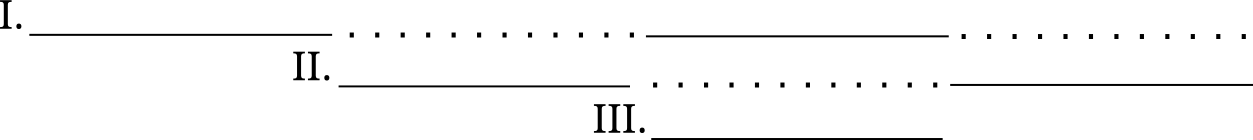
\includegraphics[height=0.6in]{propp2.png}}
\caption{Multiple simultaneous functions}\label{fig:propp2}
\end{figure}

In a typical story, one story function will follow another as the tale progresses in a sequential series of cause and effect (figure~\ref{fig:propp1}). However, Propp's formalism also allows for simultaneous story functions to be occuring at once (figure~\ref{fig:propp2}).

Though flexible, Propp's formalism is limited in its expressiveness. All story functions describe events at the same level of abstraction, describing one event after another. Also, Propp insists that the story functions occur in a prescribed order. Later French structuralists such as \citet{bremond1980logic}, \citet{greimas1983structural} and~\citet{todorov1969grammaire} address the latter problem by generalising Propp's work outside of Russian Folktales, though each represents only incremental improvements on Propp, lacking a means of nesting story functions to create abstractions. \citet{barthes1975introduction} broadly describe hierarchically composing \emph{narrative units} but, lacking implementation details, these can only be used as a template from which to build a new narrative model.
% What are the shortcomings of Propp? (i.e. lack of abstractability, etc)

% \subsection{Describing Stories with Logic}
% Laure-Ryan did a bit of this, also include linear logic approaches

\subsection{Other Types of ``Story Component''}
Lehnert's \emph{plot units} are a more recent narrative formalism
\cite{lehnert1981plot}. However, these plot units only describe stories as three
types of event: positive, negative and mental. These events occur with respect
to a single character in the story, so an author must always author story
components with concrete characters in mind, making them difficult to re-use.
Similar to Propp's system, the order of composition must always be in a certain
sequence, and plot units cannot refer to other plot units. Again, we are left
without a means of creating abstractions for our story components. In the
``TropICAL: a DSL for Tropes'' section, we address this issue by describing how tropes allow the nesting of components to allow story authors to create their own abstractions.

\section{Implementations of Experimental Narrative}
\label{sec:implementations}
% I've plenty of material, but it really needs reworking and extending

\subsection{Story Generation}
% TaleSpin, etc
Inspired by Chomsky's theories of generative grammar \citep{chomsky1968sound}, researchers in generative narrative strive to build their own `universal grammar' for narrative.

\begin{figure}[!t]
  \begin{center}
  \begin{compactenum}
    \item $\texttt{Attempt}\rightarrow \texttt{Plan} + \texttt{Application}$\\
           $\qquad\Rightarrow\texttt{MOTIVATE(Plan, Application)}$
    \item $\texttt{Application}\rightarrow\texttt{(Preaction)*} + \texttt{Action} + \texttt{Consequence}$\\
           $\qquad\Rightarrow\texttt{Allow(AND(Preaction,Preaction,...),}$\\
           $\qquad\{\texttt{CAUSE | INITIATE | ALLOW}\}\texttt{(Action,Consequence)}$
  \end{compactenum}
  \end{center}

  \caption{Example rules from Rumelhart's story grammar}\label{fig:rumelhart}
\end{figure}

\citet{rumelhart1975notes} provides one early and influential model for the grammatical generation of natural language. Figure \ref{fig:rumelhart} shows two example rewrite rules from this grammar. The `+' symbol denotes items happening in a sequence, the `\textbar' showing possible alternatives. `*' denotes one or more item being generated. Capitalised words (such as ALLOW, MOTIVATE, etc) describe relationships between items. For example, MOTIVATE is a relationship between a character's thought and their reaction to that thought.

Other systems draw inspiration from generative grammar, such as GESTER \citep{pemberton1989modular}, which generates stories based on a grammar synthesised from old French epic tales. \citet{lang1999declarative} describes a declarative model for narrative, consisting of lists of first-order predicate calculus expressions. These expressions describe events, states, goals and beliefs which combine to form a narrative. More specifically, it combines:

\begin{compactitem}
  \item A \textbf{grammar interpreter} to search for a sequence of grammar rewrites which would produce a convincing narrative.
  \item A set of \textbf{temporal predicates} to describe the occurence of events over time and enforce temporal constraints on story components.
  \item A \textbf{world model} which describes the set of actions that characters may perform and fluents that may alter over the course of the narrative.
  \item A \textbf{natural language output unit}, which takes the sequence of events produced by the story grammar and converts it into readable natural language sentences.
\end{compactitem}

This combination of using a grammar interpreter, world model and natural language output unit is especially common amongst generative grammar approaches.

While generative grammar approaches may be effective for procedurally creating
prose, they are less well suited to the creation of \emph{interactive}
narratives. Once the grammar rewrite rules are specified, the user is entirely
passive, unable to affect the way in which the story is being generated. For
this to happen, the narrative needs to be part of a system that reacts to the
actions of the user, such as in a computer game.

\begin{figure}[!t]
\begin{quote}
  ONCE UPON A TIME GEORGE ANT LIVED NEAR A PATCH OF GROUND. THERE WAS A NEST IN AN ASH TREE. WILMA BIRD LIVED IN THE NEST. THERE WAS SOME WATER IN A RIVER. WILMA KNEW THAT THE WATER WAS IN THE RIVER. GEORGE KNEW THAT THE WATER WAS IN THE RIVER. ONE DAY WILMA WAS VERY THIRSTY. WILMA WANTED TO GET NEAR SOME WATER. WILMA FLEW FROM HER NEST ACROSS THE MEADOW THROUGH A VALLEY TO THE RIVER. WILMA DRANK THE WATER. WILMA WASN'T THIRSTY ANYMORE.

GEORGE WAS VERY THIRSTY. GEORGE WANTED TO GET NEAR SOME WATER. GEORGE WALKED FROM HIS PATCH OF GROUND ACROSS THE MEADOW THROUGH THE VALLEY TO A RIVER. GEORGE FELL INTO THE WATER. GEORGE WANTED TO GET NEAR THE VALLEY. GEORGE COULDN'T GET NEAR THE VALLEY. GEORGE WANTED TO GET NEAR THE MEADOW. GEORGE COULDN'T GET NEAR THE MEADOW. WILMA WANTED TO GET NEAR GEORGE. WILMA GRABBED GEORGE WITH HER CLAW. WILMA TOOK GEORGE FROM THE RIVER THROUGH THE VALLEY TO THE MEADOW. GEORGE WAS DEVOTED TO WILMA. GEORGE OWED EVERYTHING TO WILMA. WILMA LET GO OF GEORGE. GEORGE FELL TO THE MEADOW. THE END.
\end{quote}
\caption{Example TALE-SPIN output}\label{fig:tspin}
\end{figure}

% TODO elaborate on this
James Meehan's TALE-SPIN \citep{meehan1977tale} is an influential early approach to story generation using planning. In TALE-SPIN, the author describes a story domain, its characters and their goals, and a natural language story is produced as output. It works by using a problem-solver to resolve each character's goals over the story domain. Figure \ref{fig:tspin} is an example of TALE-SPIN's output.

TALE-SPIN's strong planning component is evident in the reading of its output. Sentences are terse, with one event leading directly to another in order to achieve some goal. One problem with this character-led approach is that the goals of the author are not necessarily taken into account. If the author intends for a character to die at some point in the story, it seems unnatural for a character to have the goal of dying to fulfill this intention.

 Turner criticises TALE-SPIN's stories as seeming ``pointless and somewhat boring'' \citep{turner1986thematic}, going on to create the MINSTREL system for story generation \citep{turner1993minstrel}. Using the legendary world of King Arthur's court as a story domain, MINSTREL strives to generate stories with an authorial purpose.

MINSTREL attempts to address TALE-SPIN's shortcomings by introducing two types of schema: author-schemas and character-schemas, both of which combine to represent the elements of a story. The author-schemas describe the goals of the author of the system, allowing story creators more control over the structure and content of their narrative. This allows authors to specify a `point' or moral to their story, something that is not possible to achieve with TALE-SPIN. Character-schemas describe character-level goals in a similar manner to those of TALE-SPIN's.

The comparison of TALE-SPIN and MINSTREL highlights a challenge that has
dominated story generation for decades: the balance of \emph{character} and
\emph{plot} (as~\citet{riedl2010narrative} highlights). Especially with approaches based on multi-agent systems, the regulation of character actions to conform to an underlying theme or structure is a challenging problem.

However, modelling characters with agents is a promising approach to take in order to achieve a story which is both generative and interactive. In such a system, an author can specify the story world and character models, creating the `big picture', and the agents would be able to fill in the details (such as dialogue, sub-plots, and relationships).
An apt metaphor would be that of animation. In large animation studios such as
Disney, the lead animator draws the key frames of a sequence, and a team of
other animators work to fill in the gaps in
between\footnote{This process is described at the following website:
  \url{http://www.justdisney.com/animation/animation.html}, accessed 20160805.}. This is what the combination of a managed narrative with agents could achieve: the author would be the `lead animator' in such a system, with the agents being the assistants.

The implementations until now have focused mainly on \emph{generation\/}, and little on \emph{interaction\/}. Character models have been mentioned, but these do not react in real time to a user. For that, we need a multi-agent system.

\subsection{Characters as Intelligent Agents}
Story worlds are usually populated with characters. Interactive story worlds
such as games contain characters with very basic scripted behaviour. At even the
highest level of game character simulation, AI techniques are usually used to
govern basic behaviour such as movements and actions. Governing character
behaviour to fit within the context of a narrative is a more challenging
problem. This section examines different approaches to tackling this challenge.

\subsubsection{Planner-based Systems}
The most prevalent approach to the generation and management of plot in
interactive narrative is to use planners. With a planner, an author sets the
goals for the story (certain situations that they would like to see happen), and
the planner tells the character agents what to do to make sure these ``story
goals'' are achieved. When a player that is interacting with the system takes an
action that compromises the story goals, the planner must re-plan to make sure
the goals can still be achieved, by restricting the actions of the player or
intervening in some other manner.

% This needs elaboration
\citet{young1999notes} argues that planners are a good method for regulating
plot, later creating the \emph{Mimesis} architecture for integrating a planner with character agents in an interactive game environment, \citep{young2004architecture}. Young describes how narrative systems must re-plan when a player makes  narrative-breaking actions, by either restructuring the narrative mid-story (\emph{accommodating} the action) or preventing the action from executing (\emph{intervening} on the action).

Given its influence over subsequent approaches to interactive narrative
generation, it is worth looking at the Mimesis architecture more closely.
It is designed to integrate into the \emph{Unreal
  Tournament} game engine, and has five components: the \emph{mimesis
  controller}, the \emph{story planner}, the \emph{discourse planner}, the
\emph{execution manager} and the \emph{MWorld}.

Figure \ref{fig:mimesis} shows how these components work together to form the
Mimesis architecture. Once an author has created the pre-defined libraries of
actions needed by the story planner, the following steps are taken to determine
the course of the story:

\begin{compactenum}
  \item All the components connect to the Mimesis Controller (MC) via socket
    connection. It then acts as a message router.
  \item The game initiates a plan request containing the state of the game
    world, a list of possible actions, and the goals for the plan.
  \item The \emph{story planner} responds with a \emph{story world plan}, a data
    structure that describes the actions (selected from the list) that must occur over time in order to
    meet the plan request's goals.
  \item Once the story world plan is created, it is sent to the \emph{discourse
      planner}, along with a list of actions that can occur in the game engine
    (such as camera movements, voice-overs and background
    music). The discourse planner then creates a sequence of these actions that
    best fit the story world plan.
  \item The discourse planner then sends the narrative plan to the
    \emph{execution manager}, which builds a directed acyclic graph (DAG), where
    the nodes are the actions within the plan and the edges are the temporal
    constraints between the orderings of the actions. The execution manager
    removes nodes from the DAG in order, sends the node's actions to the
    game engine, and updates the graph.
  \item The \emph{MWorld} is essentially the environment in which the story
    occurs, consisting of the game engine, coordination code, and class
    definitions for actions, and discourse planners. It is the MWorld that
    receives actions from the execution manager to be executed, and executes
    these actions in the game engine.
\end{compactenum}

Mimesis uses DPOCL (Decomposed Partial-Order Causal-Link Planner,~\citep{young1994decomposition}) plans for
its story planning. DPOCL plans are composed of \emph{steps} (the plan's
actions), \emph{ordering constraints}, \emph{decomposition links} describing the
hierarchical structure of a plan, and \emph{causal links} between pairs of
steps. It uses \emph{refinement search} \citep{kambhampati1995planning} as its
plan reasoning process, searching through the space of possible plans represented as a directed
graph, with each node in the graph being a plan or partial plan. Mimesis
specifies the initial planning problem for DPOCL using the current and goal
states of the story.

A key feature of Mimesis is its strategies for handling of user actions which potentially
interfere with the story plan, making its goals unachievable. In the intervention strategy, Mimesis simply prevents the
user's action from having any effect in the game world. With accommodation,
Mimesis replans the story events, restructuring the plan so that the interfering
actions are taken into account and worked around.

\begin{figure}[!t]
\centerline{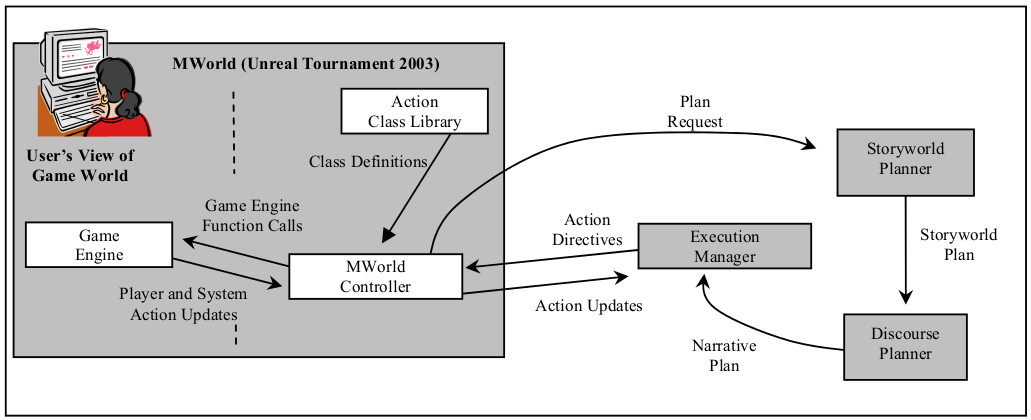
\includegraphics[height=2in]{mimesis.png}}
\caption{The Mimesis architecture, from \cite{young2004architecture}}\label{fig:mimesis}
\end{figure}

% This needs elaboration
\citet{cavazza2002character} et al's \emph{I-Storytelling} system implements
\citet{young2004architecture}'s architecture with ideas from Barthes' narrative
units~\citep{barthes1975introduction}, using characters with behaviour described
by Hierarchical Task Networks (HTNs) to generate its stories. Each character has a main task, which is divided into subtasks to create a task hierarchy, with each task node having pre- and post-conditions. The story emerges from the outcomes of each character's plans, and the narrative structure as a whole is not planned.

% This needs elaboration
\citet{riedl2003managing} describes a further development of Young's architecture,
allowing the story author to create plans for the overall narrative in addition
to its characters.
Rather than using a narrative model, this version of Mimesis models the player to track their expected level of suspense while interacting with the story. Like the \emph{I-storytelling} system, its plans are hierarchical, using the Longbow hierarchical partial-order causal link planning system~\citep{young1994decomposition}.

A disadvantage of these planner-based systems is that they require the story
author to think in a planner-oriented manner. They must consider the goals of
both the story and the character, plans to achieve these goals, and re-planning
when goals are not met or when situations change. This is a drastic change from
the usual story writing methods of authors, where the focus is on structure,
plot, themes and characters. Though graphical user interfaces such as Mimesis'
Bowman system~\citep{thomas2006author} could be used to assist plan-driven
story authoring, a complete shift in creative workflow is still required, making
this approach inaccessible to non-technical writers.

% This needs elaboration
\subsubsection{Drama manager-based Systems}

Carnegie Mellon University's OZ project \cite{mateas1999oz} uses a \emph{drama manager} to structure its narrative, which observes the actions occurring in the storyworld and ``directs'' its characters to conform to shape the story. 

Mateas and Stern's \emph{Fa\c{c}ade} has players interact with the characters of the story through natural language. In this game, the player attends the party of a young couple (Grace and Trip) celebrating their wedding anniversary. As the course of events unfold however, the player learns that all is not as happy as it seems.

The player interacts with the characters by typing in natural language sentences, to which Grace and Trip respond. Though the characters are implemented through agents, the story is controlled using a drama manager. In all, their system consists of using NLP, a novel character authoring language and a novel drama manager to create an interactive narrative.

Several custom-designed languages were used to create the game, including a language called `A Behaviour Language' (ABL) for the agents and a special language for the sequencing of the beats. ABL represents situations as character goals, maintaining a tree of all the active goals and behaviours that are happening at any time.

In Fa\c{c}ade, the smallest unit of narrative action is called a \emph{story beat}, taken from McKee's book on authorial style for screenwriters \citep{mckee1997substance}. The simulation constantly monitors what the user is doing and how it may lead from the current story beat to another. Story beats have preconditions and effects on the state of the narrative, so it is the drama manager's job to work out when it makes sense to initiate a certain beat.

`Beats' have a very fine granularity, with 200 or so updating every minute of the simulation. They consist of a set of ABL behaviours, which advance the narrative yet still allow interaction to change to other beats. Only one beat can be active at a time.

A beat can have 5 types of goal:

\begin{compactenum}
  \item transition-in: characters express their intentions
  \item body: a dramatic question/situation is posed to the player
  \item local/global mix-in: react to the player before end of the beat
  \item wait-with-timeout: wait for the player's reaction
  \item transition-out: final reaction to the player's action in the beat
\end{compactenum}

A beat goal is a series of steps for an agent to perform, which can be:

\begin{compactitem}
  \item staging (where to walk to, face)
  \item dialogue to speak
  \item where and how to gaze
  \item arm gestures to perform
  \item facial expression to perform
  \item head and face gestures to perform
  \item small arm and head emphasis motions triggered by dialogue (head nods, hand flourishes)
\end{compactitem}

As an example, there is a behaviour called ``Fix\_Drinks'', which specifies a sequence of agent behaviours where the characters Grace and Trip have an argument while Trip asks the player what they would like to drink. If the player decides not to go along with the beat (in this case, by not choosing a drink), then the beat will be aborted and replaced with another.

Fa\c{c}ade has become popular as a game outside of academia, with playthroughs of the game reaching millions of views on Youtube. This shows the promise of interactive narrative as being a unique and engaging new form of entertainment. Unfortunately, no other implementation of interactive narrative seems to have captured the public imagination since the release of Fa\c{c}ade.

Fa\c{c}ade's popularity seems to reinforce Crawford's assertion (section \ref{sec:media}) that interactive narratives must be social in nature. The gameplay comes entirely from the conversations and interactions between Grace, Trip and the player. Much of the excitement comes from the social consequences of certain conversation paths or actions. By modelling characters as agents, Mateas et al have created a truly interactive experience. However, by also using a drama manager to manage the agents, they have used these agents to tell a story.

How might these agents be made more convincing? Outside of writing rules for their behaviour consisting of character goals and beliefs, how might an author create truly unique and idiosyncratic characters? To address the question, I next examine different types of emotional models in psychology, and how each might be used to model characters as agents.

\subsubsection{Social Norms}
Versu~\cite{evans2014versu} is an interactive drama system that uses a multi agent system as characters. The characters' actions are coordinated with \emph{social practices}, which describe types of social situations and is described by the authors as a successor to the Schankian script. These social practices are implemented as reactive joint plans, which agents can choose to participate in or not. Rather than directly telling the agents what to do, these social practices merely \emph{suggest} courses of action, leaving each agent to decide for itself what to do based on its individual goals.

The authors decide against using a drama manager to control the agents' actions because they want to take the \emph{strong autonomy} approach to agent governance. This means that they prefer to give each agent some degree of autonomy by allowing it to make the final decision on which course of action to take, rather than blindly following a drama manager. Suggesting actions with social norms achieves this goal. Rather than describing typical story events in terms of social norms, however, in Versu the social norms \emph{are} the story. The gameplay revolves around the avoidance (or purposeful subvertion of) awkward social situations.

Each character has a role, which is governed by a social practice. For example, a \emph{greeting} practice involves characters with the \emph{greeter} and recipient roles. The greeting practice would tell the greeter in which manner they are to greet the recipient, and the recipient how to respond. It is noteworthy that these actions are merely suggested, and not enforced.

\emph{Exclusion logic}~\cite{evans2010introducing} is used to describe the
social practices of the system. Exclusion logic manages the frame problem by
organising related fluents in a tree structure. A single update at the right
branch can change a set of related facts en masse. For example, a description of a character called ``Brown'' is shown in listing \ref{lst:exclusive}. It describes the building up of character attributes as a tree structure.

Exclusion logic aims to address the frame problem. The frame problem is the uncertainty around whether predicates that change over time (fluents) change other predicate values. It aims to address this through use of an exclusion operator (``!''). Listing \ref{lst:exclusion} shows an example of the exclusion operator in use. The example specifies that an agent can have only one gender. The \emph{Praxis} language implementation of the exclusion logic has a type checker which ensures that no character can have multiple genders.

\begin{lstlisting}[float,label=lst:exclusion,caption=nextHopInfo: caption]
A(agent).sex!G(gender).
\end{lstlisting}

\begin{lstlisting}[label=lst:exclusion,caption=Description of ``Brown'' character.]
brown.sex!male;
brown.class!upper;
brown.in!dining_room;
brown.relationship.lucy.evaluation.attractive!40;
brown.relationship.lucy.evaluation.humour!20.
\end{lstlisting}

Exclusion logic's exclusion operator allows an author to express the fact that a variable can only have one value. For example, if `the `Brown'' character changes location from the dining room to the kitchen, \emph{brown.in!dining\_room} is terminated when \emph{brown.in!kitchen} holds.

Versu takes the \emph{constitutive} view of social practice, as opposed to the
\emph{regulative} view~\citep{SJP:SJP658}. This means that rather than restricting an agent's possible actions based on its permissions and obligations, they participate in a certain social practice by taking an action. Their actions are only restricted by what is possible in the story world, and what the agent desires to do. This way, agents can choose whether or not to take part in certain social interactions.

Many of the components we aim to have in our story telling system appear in Versu: the use of social norms to gently encourage story-conforming behaviour rather than demanding it, and the use of formal logic to determine which behaviours are possible. However in Versu the social norms \emph{are} the story, rather than describing the story components that invisibly govern the behaviour of characters. In order for this kind of governance to occur, an institution-based solution is preferable, based on events, agent actions and standard deontic logic. Because character actions are constrained by the structure of a story, a \emph{regulative}  view of social practice is more suited to the expression of story components as social norms.

Many of the advantages of using exclusion logic can be gained by using an institution-based approach. Non-inertial fluents can be used to ensure that variables can only ever have one value. Standard deontic logic is enough to provide the rest of what is needed.

% Need at least one more example here
\subsection{Modelling Narrative with Logic}
\label{sec:model-logic}
Although most recent research focuses on the use of planners to manage the drama in a story, there is also much interesting work which makes use of formal logic to model narrative. Though often used for the generation of linear story text, it is increasingly being applied to non-linear narratives as well. Logic-based approaches are generally based on either temporal logic variants or some kind of linear logic.

Ceptre~\citep{martens2015ceptre} is a language for modelling generative interactive narratives using \emph{linear logic}, a formal logic designed to describe resource usage. 

A Ceptre story begins with an initial state $\Delta_0$. Each state iteration
$\Delta_i$ is examined repeatedly, and a subset $S$ of it is updated with rule
$r$. The next state, $\Delta_{i+1}$, has the subset $S$ replaced with $S'$, the
new subset with the consequences of the applied rule $r$.

The rules are specified using the combination of logical statements with two
operators: $*$ (tensor) and $\text{-o}$ (lolli). The tensor operator is used to
concatenate statements, while the lolli operator expresses state transitions in
the form $S \mathrel{\text{-o}} S'$. The rules use \emph{replacement semantics},
which means that everything from state $S$ will disappear unless stated to be in
state $S'$. A $\$$ operator is used to mark facts in $S$ that the author wishes
to remain in $S$ without explicitly stating so.

Listing \ref{lst:ceptre-murder} shows an example from~\cite{martens2015ceptre}
that describes a ``murder'' rule and its consequences.

\begin{lstlisting}[label=lst:ceptre-murder]
do/murder
    : anger C C' * anger C C' * anger C C' * anger C C' *
    $at C L * at C' L * $has C weapon
    -o !dead C'.
\end{lstlisting}

In this case, four instances of the ``anger'' predicate with the same arguments
has a significant meaning: a character's emotion is treated as a resource. The
fact that \emph{anger $C C'$} appears four times means that a character is
\emph{four times} as angry at another character. Depending on how many times the
``anger'' statements appear in the new state, this anger can rise or fall at the
next step in the story. In this case, the emotion is not only treated as a
pre-condition, but also as a resource. These resources can also be specified
through the addition of a number to the name of the resource.

Ceptre introduces a \emph{stages} feature that allow authors to structure a
program through the use of independent components. A stage is a unit of
computation that runs to quiescence, meaning that it terminates when no more
rules are able to fire. At this point, another stage may commence.

The central motivation behind Ceptre's design is its ability to use ``proofs as
traces'', or \emph{computation as proof search}~\cite{hodas1991logic}. Ceptre
uses a \emph{sequent calculus}, where a sequent $\Delta \vdash A$, $\Delta$ is a
state, and $A$ is a goal formula. If a complete proof tree can be formed with
that sequent as its root, then the sequent can be said to be \emph{derivable}.
Thus Ceptre takes a sequent as input and creates a proof as output, declaring
failure if a proof cannot be created. Ceptre looks at the left side of the
sequent, using \emph{forward chaining} to choose which rules to try in order to
reach the goal formula.

A key feature of Ceptre is its representation of resource management in stories.
Rules are able to either produce or consume resources. This has interesting
implications for the representation of causal structure in linear logic. For
example, if two rule applications consume different sets of resources from the
same state, they are occurring concurrently and independently. However, if one
rule produces resources that are consumed by another rule, then these rules have
a causal, dependent relationship.

This modelling of gameplay as proof search is similar to the technique we use in
section~\ref{sec:thn}, where we use Interval Temporal Logic and Kripke structures to
theorem-prove certain narrative states. The difference is that the system we
describe is more concerned with representing different temporal relations,
whereas Ceptre's focus is on resource management within a game.


\subsection{Character Modelling}

\subsubsection{Characters with Emotional Models}
% Intro: not done very much?

\subsubsection{Emotional models}\label{sec:emotional-models}
% How is this useful for narrative?
Usually it would seem odd to want to model emotion as part of a computational process. Emotion is such a seemingly irrational set of behaviours that they are easy to dismiss as `human imperfections'. However, as \citet{gratch2004domain} observe, emotions may have a useful role to play in communication, so long as they are displayed at appropriate times.

For example, anger prepares the human body to fight by increasing the manufacture of adrenaline. Fear similarly triggers the `fight or flight' response, alerting the senses for danger and preparing the body to react.

In order to model human emotions using agents, we must first find a suitable psychological model to use. Marsella et al describe three main types of emotional model:

\begin{compactenum}
 \item \textbf{Discrete} emotional models, which claim that humans have a set of innate, pre-defined emotional states which people may enter and leave.
 \item \textbf{Dimensional} models of emotion, describing the spectrum of emotions as being points somewhere in continuous space. Implementations typically use two or three dimensions for simplicity.
 \item \textbf{Appraisal} theories of emotion take an agent's mental processes into account. Their emotional state is derived from whether or not their goals have been achieved, and what effects current events are having on their circumstances, for example.
\end{compactenum}

% Give examples of concrete models for each type.
\subsubsection{`Basic' emotions}
Ekman first made a case for discrete, biologically-determined emotions, based on evidence from research into facial expressions \citep{ekman1992argument}. He describes emotions as being \emph{basic}, in two senses of the word: \emph{i.} that there are a number of distinct emotions, each with its own different characteristics, and \emph{ii.} that these emotions were developed through evolution for specific functions.

Ekman argues that these evolved emotions share nine characteristics:

\begin{compactenum}
  \item Distinctive universal signals
  \item Presence in other primates
  \item Distinctive physiology
  \item Distinctive universals in antecedent events
  \item Coherence among emotional response
  \item Quick onset
  \item Brief duration
  \item Automatic appraisal
  \item Unbidden occurrence
\end{compactenum}

These characteristics are shared by all of the `basic' emotions as observed in humans and primates.

Discrete models of emotion suggest that there is a neural basis for emotion. For example, Armony et al describe how the amygdala in the brain is responsible for conditioned fear responses  and create a neural network to model it \citep{armony1997computational}.

Using a discrete model of emotion for agent-based characters would be relatively simple. Each basic emotion could have its own distinct set of behaviours as postconditions, and triggering circumstances as preconditions.

However, a more fluid approach could be useful when modelling emotions with agents. It would be impossible to say that an agent is \emph{angry and approaching furious} using a discrete theory of emotion. Nuanced levels of emotion and even combinations of several emotions add an extra level of texture to a character. Dimensional and appraisal theories of emotion address this challenge.

\subsubsection{Russell's circumplex model of emotion}\label{sec:circumplex}
\begin{figure}[!t]
\centerline{
\includegraphics[height=3in]{circumplex.png}}
\caption{Russell's circumplex model of emotion} \label{fig:circumplex}
\end{figure}

Russell's circumplex model of emotion is a well-known dimensional model \citep{russell1980circumplex}. In this case, the dimensional variables are \emph{valence} (how agreeable or otherwise a situation is to an agent) and \emph{arousal} (how excited an agent is).

Russell's original paper proposes a model similar to that shown in figure \ref{fig:circumplex}, where the $x$ axis is a person's valence level and the $y$ axis is their arousal level. He argues that the full range of human emotions lie as points along these axes. Eight such examples are shown in fig. \ref{fig:circumplex}.

This model is very easy to adapt to human-like agents. \citet{ahn2012nvc} adapt this model by adding a third dimension, dominance, to create conversational agents in a 3D environment. This `dominance' dimension was first proposed in Mehrabian and Russell's original work \citep{mehrabian1974approach}, but later removed due to being perceived as the consequences of the \emph{effects\/} of emotion \citep{russell1980circumplex}, rather than being a component of emotion itself. Like Ahn et al, I found it useful to add the dominance-submission dimension, and so left it in my emotional model. This is the approach I take in creating my Punch and Judy simulation, and so it is described in more detail in section \ref{sec:emotion}.

\subsubsection{Appraisal theory}
Appraisal theories of emotion lend well to simulation with agents, due to their taking a person's beliefs, desires and intentions into account with respect to external events. Emotions arise when an event occurs and a person internally \emph{appraises} its consequences with respect to their beliefs, desires and intentions. This fits well with the popular BDI architecture for intelligent agents.

Different methods of appraisal may be used in order to produce emotions. Gratch and Marsella use decision theoretic plans \citep{gratch2004domain}, but other approaches could include reactive plans, Markov-decision processes, or detailed cognitive models.

Though the Punch and Judy simulation described in section \ref{sec:punchjudy} uses a dimensional model of emotion, an appraisal-based model would be worth investigating due to its tight coupling with belief desire intention psychological models used in agents. I describe my intention to explore this area further in section \ref{sec:fappraisal}.

\subsection{Discussion}\label{sec:litrev-discussion}
Through this literature review, we have clearly identified these main issues in
need of attention:

\subsubsection{Character agents need some freedom to generate story details}
In most of the systems described in this literature review, the agents in a
story world are explicitly told what to do.

% Based on the analysis above, we hypothesise that using social institutions to
% govern the actions of character agents allows for more flexibility in the
% agents' actions. By 

\subsubsection{Story authors do not want to think in terms of goals}
The current dominant paradigm in interactive narrative creation is to
use planners to ``plan'' a narrative, and re-plan when a user interacts in
an unexpected manner. This does not align well with non-programmer story
authors, who are likely to be unfamiliar with planning systems. In order to
create these stories with planners, they would have to think of the story in
terms of story and character goals.
\subsubsection{Most narrative systems use outdated, inflexible story models}
There is an over-reliance on narrative formalisms such as
Propp~\citep{propp1968morphology} even in recent narrative generation
systems. Neither narrative nor AI research have produced a formalism for
narrative components that has endured. This is likely because Propp's formalism
is ``good enough'', and has worked for most researchers that have used it. There
is also likely to be a network effect, where Propp has become the formalism that
most researchers have heard of, and therefore the one that they end up using.

Though there have been attempts to create more expressive formalisms as
described in section~\ref{sec:formalisms}, none have been expressive enough to
overcome Propp's ``good enough'' properties. In order for a story model to
significantly improve upon Propp, it should add features that it and other
existing formalisms lack. We identify these features as:

\begin{compactitem}
  \item A means of \emph{abstraction}
  \item Conceptually \emph{simple} enough for non-programmers to grasp
  \item A library of re-usable \emph{examples} for authors and researchers
\end{compactitem}

\paragraph{A Means of Abstraction}
Current narrative formalisms lack a means of \emph{abstraction}. Propp,
for example, describes events in stories that all occur at the same level of
abstraction. This means that one is limited to describing events that occur one
after another, or in parallel, but not events that contain sub-events.

For example, suppose we define a ``Quest'' component of a story, which describes a
sequence of events that occur (such as the hero leaving home and then defeating
a monster). It is easy to think of other story components that could contain
this ``Quest'' component, such as ``Hero's Journey'', ``Rescue the World'' or
``Rite of Passage'' story components. These components could themselves be used
as part of other components. This gives us a means of creating abstractable,
reusable story components. Of all the story models described in
section~\ref{sec:formalisms}, none have any means of abstraction such as this.

The example we just described already hints at the use of story tropes that
contain other tropes. This is the means of abstraction and re-use that we use in
our system, described in section~\ref{sec:tropes}.

\paragraph{Conceptually Simple}
Story authoring tools are user interfaces which are used to write fiction. In
the computing world, user interfaces are often simplified through the use of an
\emph{analogy}. For example, a \emph{Desktop Environment} is a graphical user
interface analogy created by Xerox in the 1970s. Where computer users would
previously have had to learn and master a complicated command-line interface,
the desktop environment metaphor presented an interface that resembled something
that users were already familiar with: the top of a desk, with icons
representing files spread out over a ``desktop'' surface.

When creating a story model, it is easy to fall into the trap of creating
something complicated but arbitrary. As with Vonnegut's ``Shapes of Stories''
metaphor (described in section~\ref{sec:shapes}, sometimes the simplest
explanations are the easiest to grasp and most enduring. We believe that our
``trope'' analogy for modelling stories (section~\ref{sec:tropes}) is an
elegant, expressive and accessible way of describing parts of stories using a formalism.

Most story authors are already familiar with the concept of tropes. When
questioned about their familiarity with the idea, all the participants at an
interactive fiction meetup responded that they were familiar with the ``trope''
concept (sample size 19, see section~\ref{sec:tropes-simple}). This means that tropes are a
suitable analogy for the creation of a new narrative formalism.

\paragraph{A Library of Re-usable Examples}
Part of the problem of existing formalisms is that story authors that use them
need to write their own story components based on a formalism's description.
Though these formalisms are usually described in papers with one or two
examples, any story author would have to create their own formal descriptions,
even for commonly-occuring story components such as quests or \emph{The Hero's
  Journey}. What is needed is a library of pre-existing formal descriptions of
story components that authors can easily copy and paste into their stories.

As the concept of \emph{tropes} is one that is already well-known to story
authors and consumers of media, it is easy to find many examples of them in
reviews of books, films and computer games. In fact, there is a whole website
called ``TV Tropes'', which is dedicated entirely to the description of tropes
that recur throughout different types of media. This website takes the form of a
wiki, with a very active community who contribute trope descriptions along with
lists of the media they appear in.

For example, a trope called ``Karma Houdini'' has the following description:

\begin{quote}
The character has done a number of things that deserve a karmic comeuppance,
most importantly things that caused harm to the innocent.
But when the time comes for the hammer to fall, that's not what happens. At
least, not on him.
He doesn't get what he deserves. Instead, he gets away scot-free.
And he might even have reversed the Humiliation Conga that was being planned for him.

This is it. This is all there is to the story. The show is over. The book is finished. The author isn't going to write any more. The Word of God has been spoken. The guy has become a Karma Houdini.
\end{quote}

The site lists many examples from film and literature, including:
\begin{compactitem}
  \item \textbf{Treasure Island:} Long John Silver escaped scot free with a chest of treasure, and was never caught. Not bad, for a month's murder and betrayal.
  \item \textbf{The Talented Mr Ripley:} Villain Protagonist Tom Ripley killed some people to assume a new identity and enrich himself thoroughly. In the sequels, he killed to protect his new life, and sometimes as favors for others. He never faced justice.
\end{compactitem}

The \emph{TV Tropes} website is a Wikipedia of sorts for tropes. Since there are
already so many examples listed on its website, it reduces the work needed to
create a library of reusable formal descriptions of tropes. We have created such
a library, which is described in section~\ref{sec:library}.

These three omissions (means of abstraction, conceptual simplicity and a
re-usable library of components) from existing narrative systems are addressed
by our trope-based approach to interactive narrative generation, which is
described in further sections of this thesis. Section~\ref{sec:tropes} describes
the trope concept further, with examples. Section~\ref{sec:institutions}
explains how these tropes are used to govern agents in a multi-agent system. We
describe TropICAL, our domain-specific language for tropes, in
section~\ref{sec:tropical}. Section~\ref{sec:library} describes our creation of
a library of tropes and section~\ref{sec:policy} describe the application of our
\emph{tropes} concept to legal policies. The thesis concludes with an evaluation
in section~\ref{sec:evaluation} and conclusions in section~\ref{sec:conclusions}.

\include{current}
\include{plan}

\bibliographystyle{apalike}
\bibliography{thesis}

\end{document}